\section{Precise-Alignment Pipeline}
\label{sec:precise-alignment-methodology}

The relocalisation pipeline described in this section refines the coarse initial pose estimate delivered by the SLAM system presented in \cref{chap:SLAM} through point cloud registration against a pre-built 3D Gaussian Splatting reference model. Two independent sensing modalities, stereo vision and accumulated LiDAR, are evaluated within a common architectural framework; both feed into a shared ICP registration backend, the output of which is used to correct the robot's estimated pose in the ROS~2 transform tree. The approach is outlined in \cref{subsec:approach-overview}; the following subsections present each component in detail.

% ---------------------------------------------------------------
\subsection{System Overview}
\label{subsec:pa-system-overview}
% ---------------------------------------------------------------

The precise-alignment pipeline operates as a one-shot refinement: when the robot halts in front of a target vine, a single localisation correction is computed and applied before any manipulation motion is initiated. The pipeline consists of three cooperating components: a sensor-specific preprocessing stage that transforms raw sensor data into a filtered, downsampled point cloud; a target cloud extraction stage that constructs a single reference point cloud directly from the Gaussian mean positions of the 3DGS model; and a shared GICP registration stage that searches for the optimal rigid alignment between the sensor observation and the extracted reference across 35 perturbation hypotheses sampled around the initial pose. The corrected pose is subsequently propagated to the robot's transform tree without modifying the SLAM system's own published transforms.

Two independent sensing modalities are evaluated. The stereo vision pipeline accepts rectified image pairs from two ZED stereo cameras, applies the FoundationStereo foundation model~\cite{wenFoundationStereoZeroShot2025}
to estimate dense disparity maps, and derives coloured 3D point clouds that are segmented to retain vine trunk structure. The LiDAR pipeline operates on dense point clouds accumulated from a Livox Mid-360 LiDAR over a set interval, using Patchwork++ for ground plane removal, and applying a multi-stage filtering sequence to clean up and isolate the vine. Both pipelines share the same GICP registration module and the same pose correction mechanism; they differ only in their preprocessing steps, which are tailored to the noise characteristics and geometric coverage of the respective sensor. 

The initial pose estimate consumed by the pipeline is provided by the SLAM system described in \cref{sec:slam-methodology}. This pose locates the robot within the global coordinate frame and is used to generate initial transform perturbation hypotheses for GICP registration, as well as to anchor the final corrected transform in the global frame. The pipeline dataflow for each sensing modality is illustrated in
\cref{fig:pa-pipeline-stereo,fig:pa-pipeline-lidar}; the shared GICP
registration stage is shown in \cref{fig:pa-pipeline-icp}.

\begin{figure}[htbp]
  \centering
  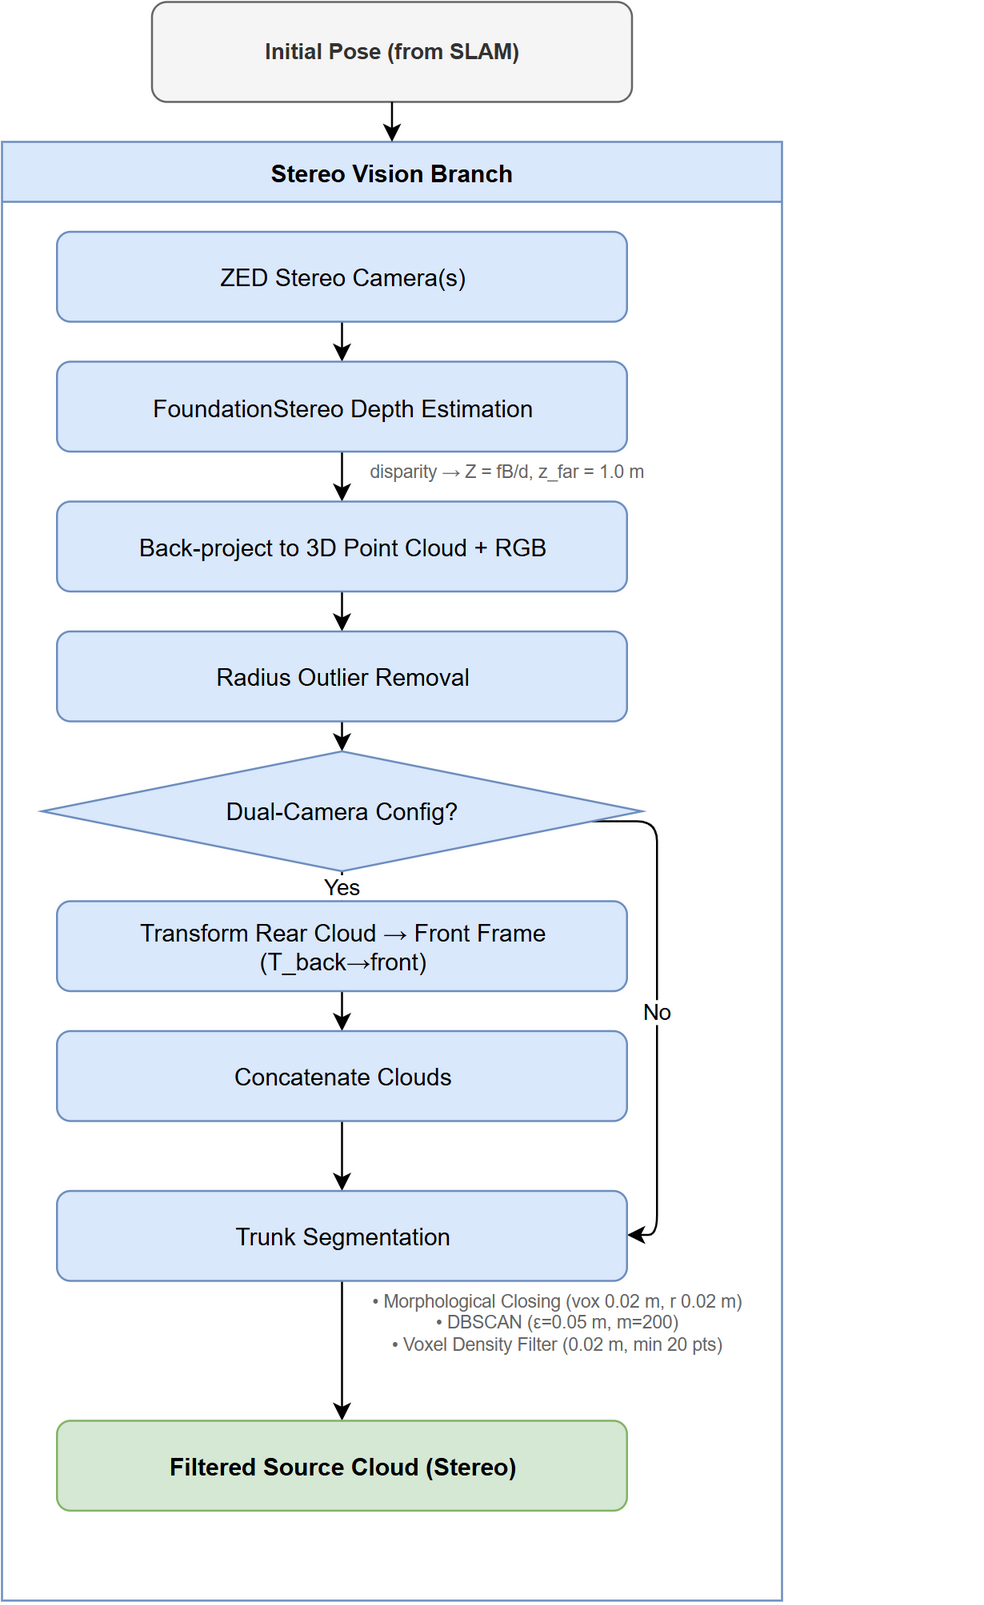
\includegraphics[width=0.65\linewidth]{4-precise-alignment/4-methodology/figures/pa-pipeline-stereo}
  \caption{Stereo vision preprocessing branch of the precise-alignment pipeline.
           Rectified image pairs from the ZED stereo camera(s) are processed
           through FoundationStereo depth estimation, back-projection, radius
           outlier removal, optional dual-camera fusion, and trunk segmentation
           to produce a filtered source point cloud passed to the shared GICP
           registration stage (\cref{fig:pa-pipeline-icp}).}
  \label{fig:pa-pipeline-stereo}
\end{figure}

\begin{figure}[htbp]
  \centering
  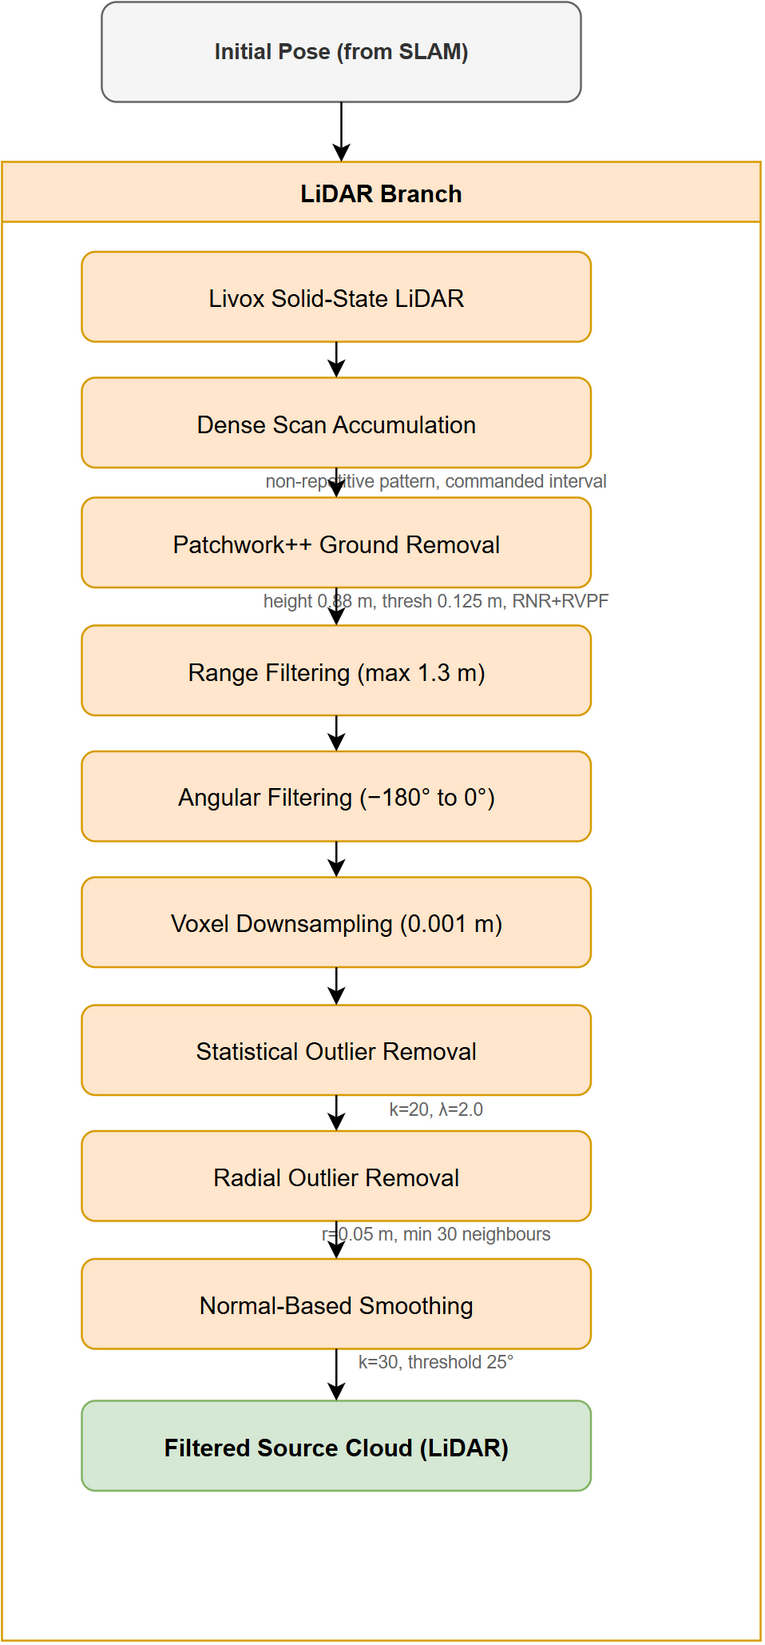
\includegraphics[width=0.65\linewidth]{4-precise-alignment/4-methodology/figures/pa-pipeline-lidar}
  \caption{LiDAR preprocessing branch of the precise-alignment pipeline. Dense
           scans from the Livox solid-state LiDAR are filtered through ground
           removal, statistical and angular outlier rejection, and normal-based
           smoothing to produce a filtered source point cloud passed to the
           shared GICP registration stage (\cref{fig:pa-pipeline-icp}).}
  \label{fig:pa-pipeline-lidar}
\end{figure}

\begin{figure}[htbp]
  \centering
  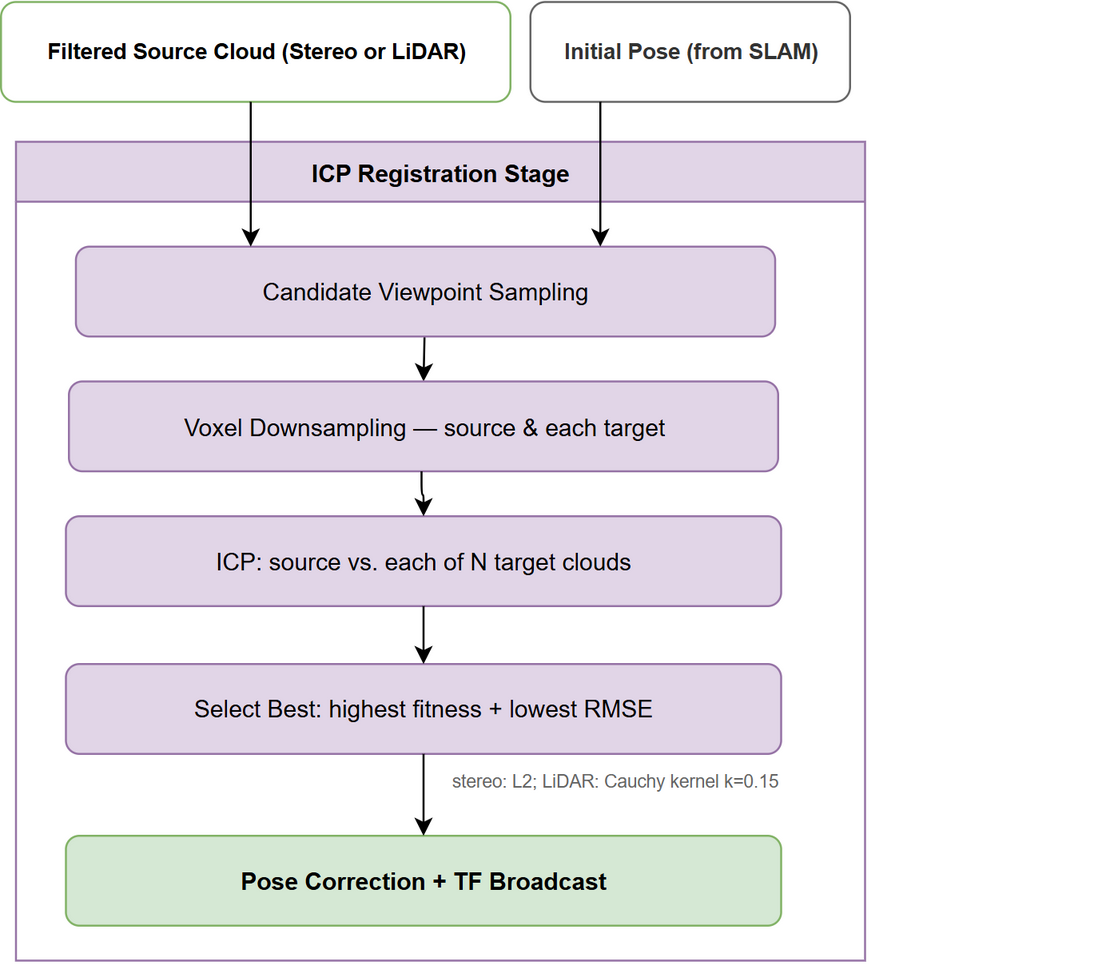
\includegraphics[width=0.85\linewidth]{4-precise-alignment/4-methodology/figures/pa-pipeline-icp}
  \caption{Shared GICP registration stage, common to both sensing modalities.
           A single target point cloud is extracted from the Gaussian mean
           positions of the 3DGS model; 35 perturbation hypotheses are sampled
           around the initial SLAM pose and each is registered via GICP against
           the extracted target cloud. The best-fitting result is used to correct
           the robot pose in the ROS~2 TF tree via the mechanism described in
           \cref{subsec:pa-pose-correction}.}
  \label{fig:pa-pipeline-icp}
\end{figure}

% ---------------------------------------------------------------
\subsection{Reference Model: 3D Gaussian Splatting}
\label{subsec:pa-reference-model}
% ---------------------------------------------------------------

The localisation target for both sensor modalities is a point cloud derived directly from the 3DGS model of the target vine. The construction of this model from SfM photogrammetry is described in \cref{subsec:system-context}; the present subsection addresses how it is used during localisation.

The 3DGS model is loaded once at initialisation. The target point cloud is constructed by extracting the mean positions of all Gaussian primitives stored in the model. Each primitive is parameterised by a mean $\boldsymbol{\mu}_i \in \mathbb{R}^3$, representing the centre of the volumetric Gaussian in world coordinates; collecting these centres across all $N$ primitives yields a single global point cloud $\{\boldsymbol{\mu}_i\}_{i=1}^{N}$ that captures the geometric structure of the reconstructed scene (see \cref{fig:pa-gaussian-splat-pointcloud}). This extraction is a direct read of the model parameters and requires no rendering pass, making it computationally simpler than viewpoint-dependent depth map synthesis and free of viewpoint-dependent artefacts that arise when projecting volumetric primitives onto an image plane.

Because the extracted cloud spans the full reconstructed scene, it is spatially cropped to a region of interest centred on the initial pose estimate before registration. This step retains only the local geometry relevant to the current alignment problem and discards distant or structurally irrelevant model points that would otherwise inflate correspondence search cost and introduce spurious matches. Following cropping, the target cloud may optionally be downsampled using a voxel grid filter to reduce point density and match the resolution of the incoming sensor source cloud, further reducing the computational cost of the subsequent registration step.

The resulting target cloud is constructed once per localisation query and reused across all perturbation hypotheses evaluated during ICP registration, as described in \cref{subsec:pa-icp-registration}. This avoids redundant reconstruction overhead and ensures a consistent geometric reference throughout the alignment procedure.

\begin{figure}[htbp]
  \centering
  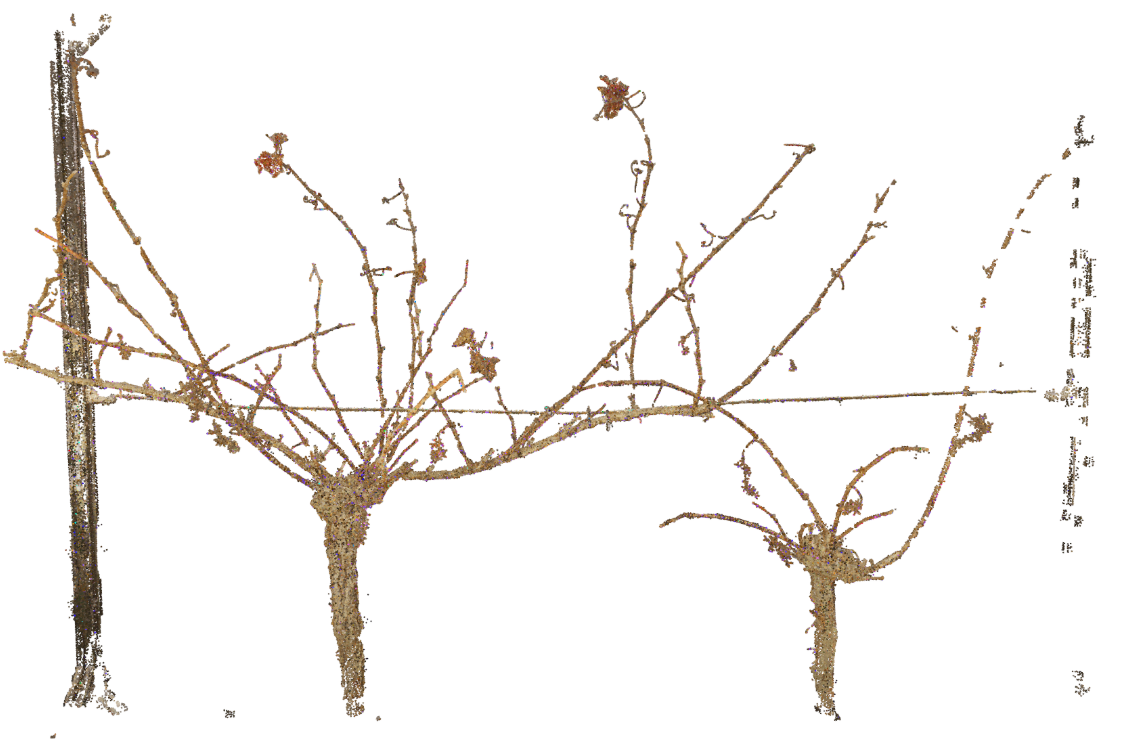
\includegraphics[width=0.85\linewidth]{4-precise-alignment/4-methodology/figures/pa-gaussian-splat-pointcloud}
  \caption{Point cloud derived from the 3DGS reference model of a dormant
           grapevine, constructed by extracting the mean positions
           $\boldsymbol{\mu}_i$ of all Gaussian primitives. Two vine trunks
           and the shared trellis wire are clearly resolved.}
  \label{fig:pa-gaussian-splat-pointcloud}
\end{figure}

% ---------------------------------------------------------------
\subsection{Stereo Vision Pipeline}
\label{subsec:pa-stereo-pipeline}
% ---------------------------------------------------------------

The stereo vision pipeline converts raw rectified image pairs from the ZED stereo camera into a filtered point cloud of the vine trunk, for registration against the 3DGS target described in \cref{subsec:pa-reference-model}. The pipeline proceeds through three sequential stages: dense depth estimation from the stereo pair, optional fusion of point clouds from a laterally offset camera pair, and trunk segmentation to remove non-structural points. The output is passed directly to the shared ICP registration stage described in \cref{subsec:pa-icp-registration}.

\subsubsection{Depth Estimation}
\label{subsubsec:pa-depth-estimation}

Dense depth estimation is performed using FoundationStereo~\cite{wenFoundationStereoZeroShot2025},
a stereo foundation model that produces disparity maps with strong zero-shot generalisation across sensor configurations and scene types (see \cref{subsec:stereo-depth} for a description of the model and its benchmark performance).
The \texttt{23-51-11} checkpoint is used without any fine-tuning; inference is applied in a purely zero-shot manner.
FoundationStereo is applied to rectified image pairs from the ZED Mini stereo camera. Prior to inference, the input images are downscaled by a factor of 0.7 relative to the original sensor resolution.
This factor was determined empirically: the largest input resolution that can be processed without exceeding available GPU memory was identified, and a 20\,\% safety margin was applied, yielding the 0.7 scale factor.

The disparity map produced by FoundationStereo is converted to metric depth via the standard pinhole relation (see \cref{subsec:stereo-depth}):
%
\begin{equation}
    Z = \frac{f \cdot B}{d},
\end{equation}
%
where $Z$ is the metric depth, $f$ is the focal length of the rectified camera model, $B$ is the stereo baseline, and $d$ is the estimated disparity at each pixel. A far-clip distance of $z_\mathrm{far} = 1.0$\,m is applied to discard depth estimates beyond the typical operating range between the robot and the target vine.
% TODO: review justification: z_far = 1.0 m reflects the close-range operating distance in the vineyard row; review against actual deployment geometry
Points with depth below a minimum threshold are also discarded to suppress artefacts close to the camera aperture.

Each pixel for which a valid depth estimate is available is back-projected into a three-dimensional point in the camera frame, using the corresponding RGB values to produce a coloured point cloud. A radius outlier removal filter is subsequently applied to eliminate sparse, isolated points that are not part of any coherent surface.

\subsubsection{Dual-Camera Point Cloud Fusion}
\label{subsubsec:pa-dual-camera}

The system supports an optional dual-camera configuration in which a second ZED stereo camera (ZED~2) is mounted alongside the primary camera (ZED~1) on the vine-facing side of the robot platform, approximately 30\,cm laterally offset with no rotation between the two units. Both cameras are directed toward the same face of the vine structure, producing overlapping point clouds from slightly different lateral vantage points.

This configuration serves two complementary purposes. First, the lateral offset provides marginally different viewing angles of the vine surface, yielding a denser and more representative composite point cloud than either camera alone. Second, points in the shared field of view are observed from two independent viewpoints and therefore accumulate higher local density after concatenation; this is passively exploited by the downstream density-sensitive filters described in \cref{subsubsec:pa-trunk-segmentation}, which preferentially retain the denser overlap region over sparse peripheral returns. No explicit consistency-based outlier rejection is applied in the current implementation. Flagging depth estimates that appear in one cloud but are absent or inconsistent in the other would represent a more deliberate exploitation of the overlap, and remains a potential avenue for improvement. This stands in contrast to a configuration in which the two cameras view the vine from opposite or widely separated directions, where each cloud would have to be accepted independently with no means of cross-validation.

The extrinsic relationship between the two cameras is expressed as a rigid transform from the secondary camera frame (ZED~2) to the primary camera frame (ZED~1). Given the transform from the primary camera to a common reference frame, $T_{\mathrm{cam1} \to \mathrm{ref}}$, and the corresponding transform from the secondary camera, $T_{\mathrm{cam2} \to \mathrm{ref}}$, the inter-camera transform is computed as:
%
\begin{equation}
    T_{\mathrm{cam2} \to \mathrm{cam1}} = T_{\mathrm{cam1} \to \mathrm{ref}}^{-1} \cdot T_{\mathrm{cam2} \to \mathrm{ref}}.
    \label{eq:dual-camera-extrinsic}
\end{equation}
%
The secondary camera point cloud is transformed into the primary camera frame using $T_{\mathrm{cam2} \to \mathrm{cam1}}$, and the two clouds are concatenated (\cref{fig:pa-dual-camera}). Since both cameras share the same pointing direction, the rotation component of $T_{\mathrm{cam2} \to \mathrm{cam1}}$ is the identity in the nominal configuration, reducing the transform to a pure lateral translation of approximately 30\,cm.

\begin{figure}[htbp]
  \centering
  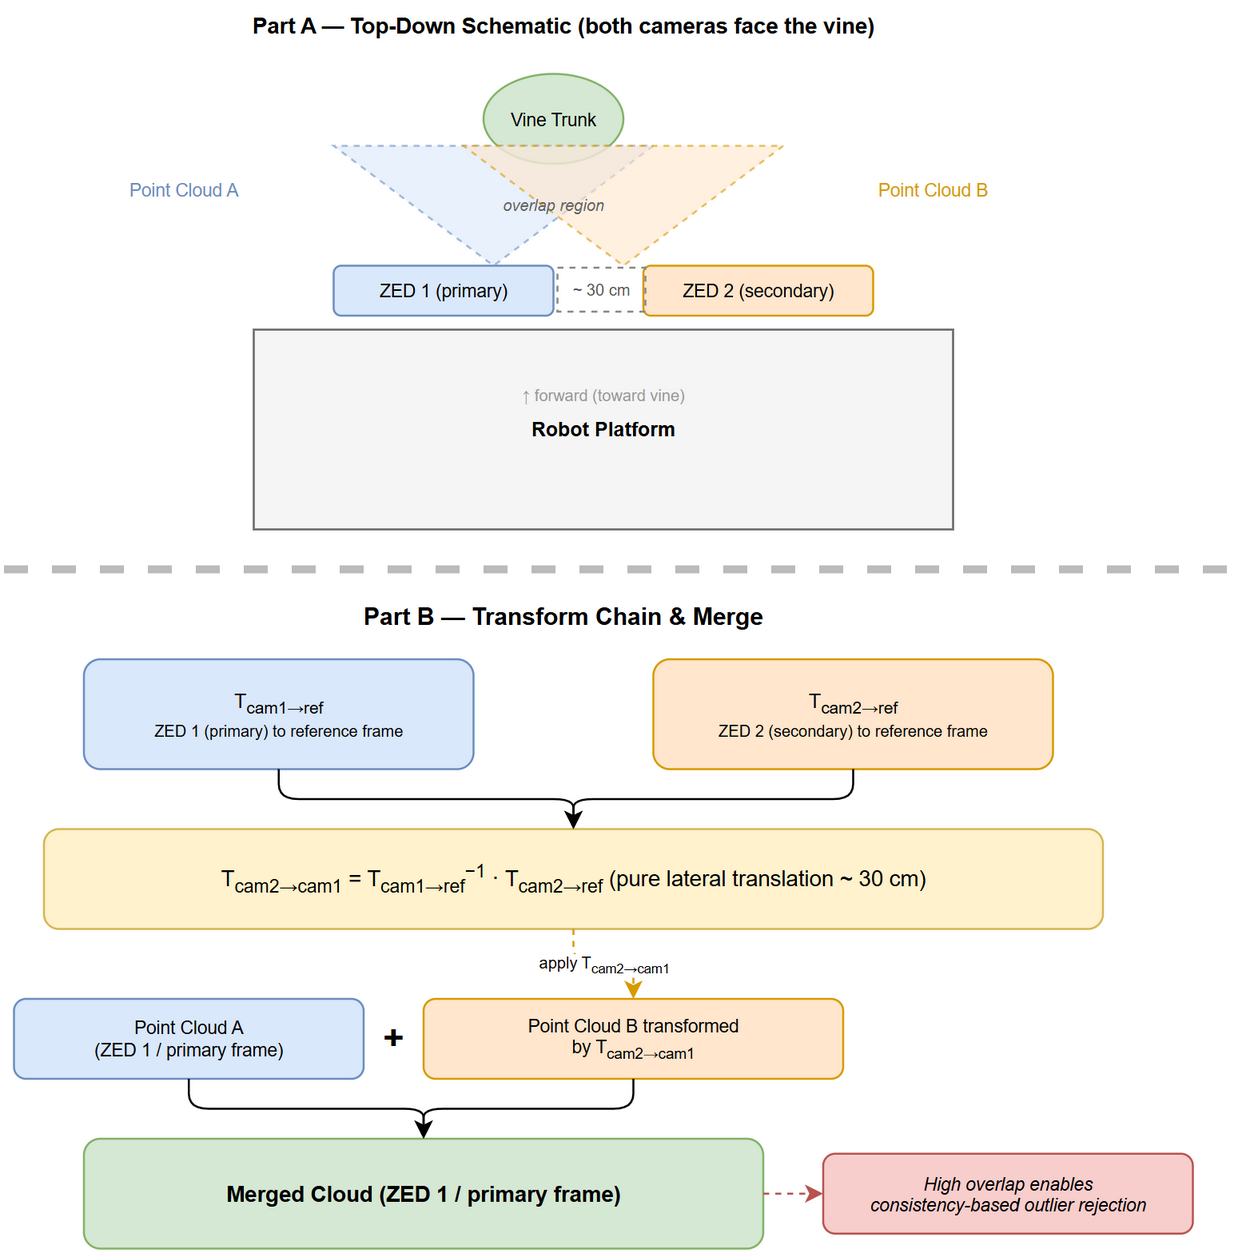
\includegraphics[width=\linewidth]{4-precise-alignment/4-methodology/figures/pa-dual-camera}
  \caption{Dual-camera point cloud fusion. Both ZED cameras are mounted side by side
           on the vine-facing side of the robot, approximately 30\,cm apart with no
           rotation between them, and directed toward the same face of the vine (Part~A).
           The secondary camera's point cloud is transformed into the primary camera
           frame using $T_{\mathrm{cam2} \to \mathrm{cam1}}$ (\cref{eq:dual-camera-extrinsic}),
           and the two clouds are concatenated (Part~B). The resulting overlap region
           accumulates higher local point density, which is passively exploited by the
           downstream density-sensitive filters in the trunk segmentation stage.}
  \label{fig:pa-dual-camera}
\end{figure}

\subsubsection{Trunk Segmentation}
\label{subsubsec:pa-trunk-segmentation}

A custom trunk segmentation pipeline developed for this work is applied to the merged (or single-camera) point cloud to isolate the vine trunk from background vegetation, noise, and ground returns; the three sequential stages are summarised in \cref{fig:pa-trunk-segmentation}.

\begin{figure}[htbp]
  \centering
  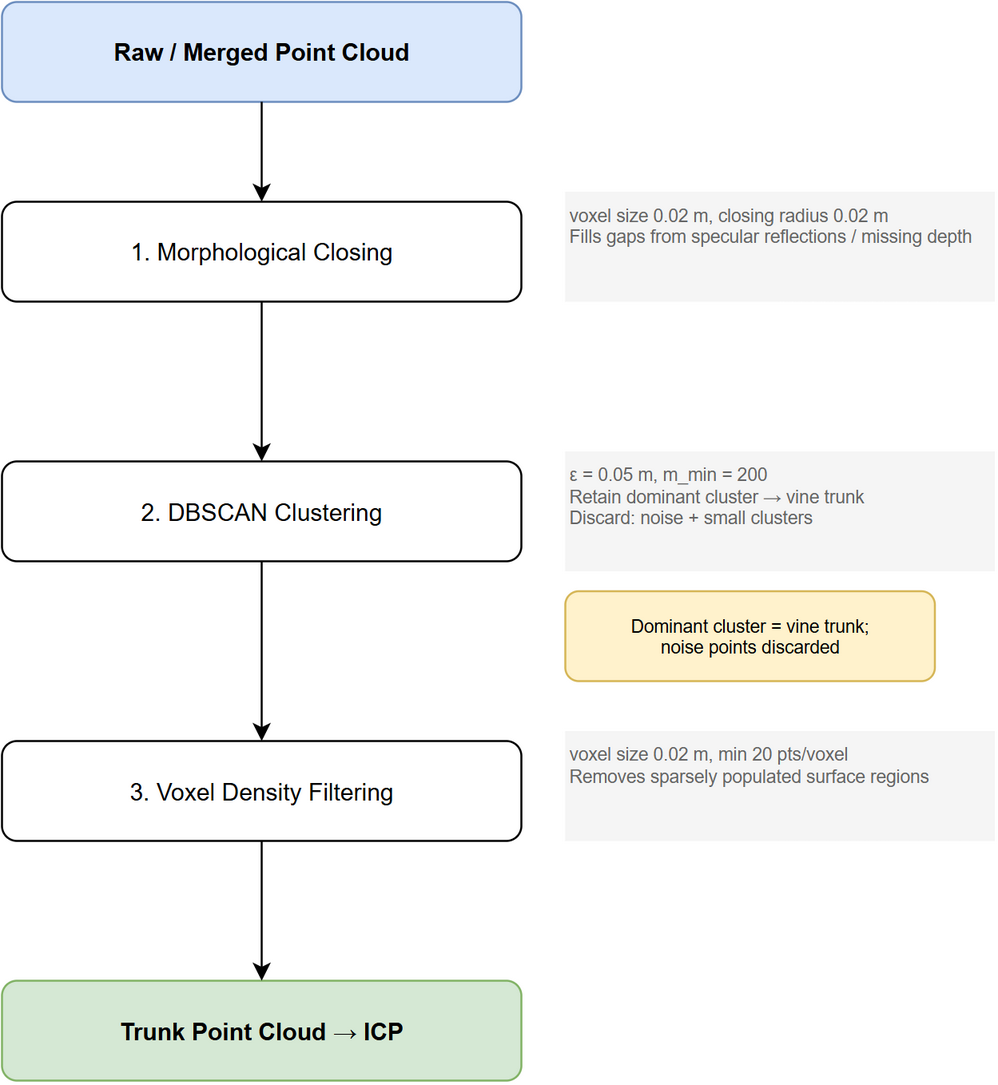
\includegraphics[width=0.75\linewidth]{4-precise-alignment/4-methodology/figures/pa-trunk-segmentation}
  \caption{Stereo trunk segmentation pipeline. The merged point cloud passes through
           three sequential stages (morphological closing, DBSCAN clustering, and
           voxel density filtering) to isolate the vine trunk from background
           vegetation, ground returns, and noise.}
  \label{fig:pa-trunk-segmentation}
\end{figure}

The pipeline comprises three sequential stages. Prior to the first stage, the combined cloud is capped at 600,000 points by random subsampling, bounding the worst-case computation time independently of sensor resolution or accumulation duration.
% TODO: review whether 600,000 is the tightest practical cap; review against observed input sizes

\textbf{Morphological closing.} A voxel-based morphological closing operation fills gaps in the trunk surface caused by specular reflections or missing depth estimates. The input cloud is voxelised at a resolution of 0.02\,m, and a spherical closing kernel of radius 0.02\,m is applied.
% TODO: review parameter justification: voxel size 0.02 m and closing radius 0.005 m were selected to bridge typical surface gaps in stereo depth reconstructions of vine bark; review against observed gap statistics

\textbf{DBSCAN clustering.} Density-Based Spatial Clustering of Applications with Noise (DBSCAN)~\cite{esterDensityBasedAlgorithmDiscovering1996}
partitions the closed point cloud into spatially coherent clusters. DBSCAN groups points whose neighbourhood within radius $\varepsilon$ contains at least $m_\mathrm{min}$ neighbouring points, classifying the remainder as noise. With $\varepsilon = 0.05$\,m and $m_\mathrm{min} = 200$,
% TODO: review parameter justification: eps = 0.05 m reflects the typical inter-point spacing at vine-trunk distances; min_samples = 200 was chosen to reject small noise clusters while retaining the dominant trunk; review against cloud density statistics
the dominant cluster, corresponding to the vine trunk, is retained, and all other clusters and noise points are discarded.

\textbf{Voxel density filtering.} The retained cluster is passed through a voxel density filter that partitions the cloud into voxels of side length 0.02\,m and discards any voxel containing fewer than 20 points.
% TODO: review parameter justification: voxel size 0.02 m and min count 20 eliminate residual sparse regions that survived clustering; review against observed point density at typical vine-to-sensor distances
This step removes sparsely populated surface regions whose geometric contribution to the ICP objective would otherwise be disproportionate to their informational content.
\Cref{fig:pa-stereo-pointcloud-processing} illustrates the effect of the full stereo preprocessing pipeline on a representative observation.

\begin{figure}[htbp]
  \centering
  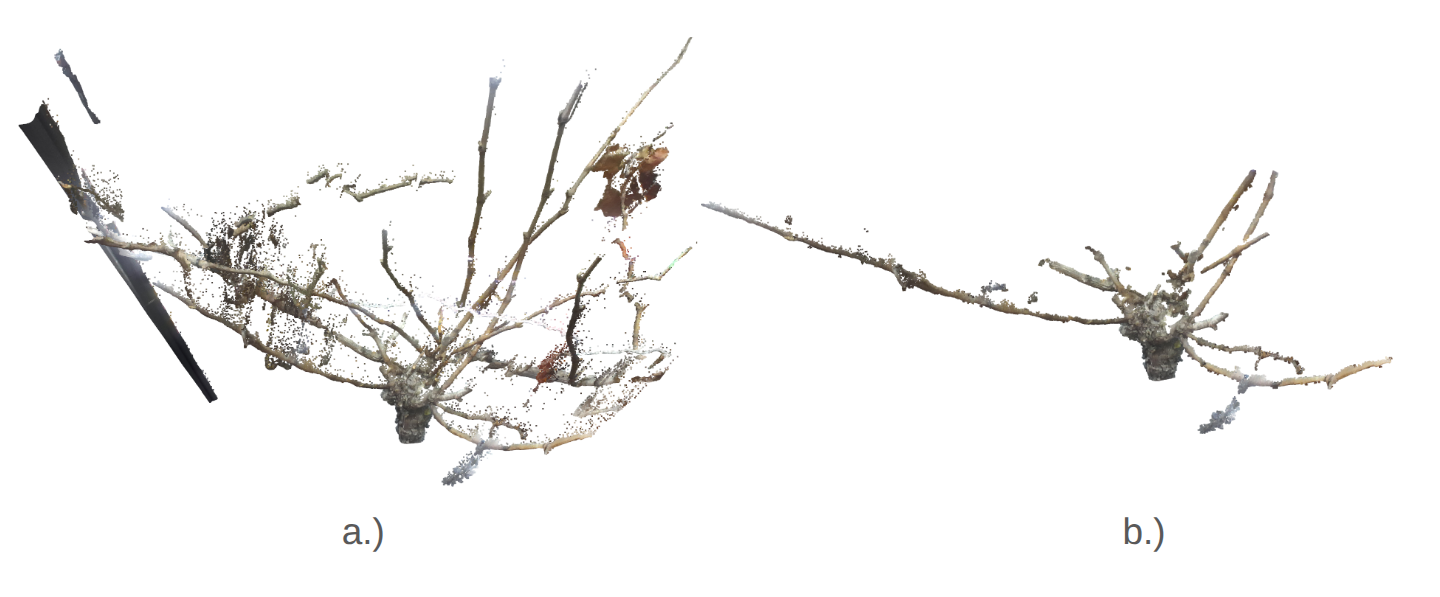
\includegraphics[width=\linewidth]{4-precise-alignment/4-methodology/figures/pa-stereo-pointcloud-processing}
  \caption{Stereo point cloud before and after preprocessing.
           (a) The raw back-projected point cloud prior to filtering, exhibiting
           significant noise, non-structural returns, and artefacts.
           (b) The filtered point cloud following the full trunk segmentation
           pipeline, retaining only the vine trunk geometry forwarded to GICP
           registration.}
  \label{fig:pa-stereo-pointcloud-processing}
\end{figure}

The parameters for the stereo preprocessing pipeline are summarised in \cref{tab:pa-stereo-params}.

\begin{table}[htbp]
  \centering
  \caption{Stereo vision pipeline parameters.}
  \label{tab:pa-stereo-params}
  \begin{tabularx}{\textwidth}{l l X}
    \toprule
    \textbf{Parameter} & \textbf{Value} & \textbf{Description} \\
    \midrule
    Downscale factor          & 0.7        & Input image downscale factor for FoundationStereo inference; empirically derived with a 20\,\% GPU memory safety margin \\
    $z_\mathrm{far}$          & 1.0\,m     & Far-clip depth; points beyond this distance are discarded \\
    Closing voxel size        & 0.02\,m    & Voxel resolution for the morphological closing operation \\
    Closing radius            & 0.02\,m    & Spherical kernel radius for the closing operator \\
    DBSCAN $\varepsilon$      & 0.05\,m    & Neighbourhood radius for cluster membership \\
    DBSCAN $m_\mathrm{min}$   & 200        & Minimum point count to form a core cluster \\
    Density filter voxel size & 0.02\,m    & Voxel size for the density filtering stage \\
    Density filter min count  & 20         & Minimum points per voxel \\
    Input point cap           & 600\,000   & Maximum points admitted to the segmentation pipeline \\
    \bottomrule
  \end{tabularx}
  % TODO: verify all parameter values and add justifications
\end{table}

% ---------------------------------------------------------------
\subsection{LiDAR Pipeline}
\label{subsec:pa-lidar-pipeline}
% ---------------------------------------------------------------

The LiDAR pipeline converts raw scans from the LiDAR into a filtered point cloud of the vine structure, ready for registration. The pipeline proceeds through three stages: dense scan accumulation to build a spatially rich input cloud, ground plane removal using Patchwork++, and sequential geometric filtering. The output is dispatched to the shared ICP registration stage described in \cref{subsec:pa-icp-registration}.

\subsubsection{Dense Scan Accumulation}
\label{subsubsec:pa-dense-accumulation}

The Livox Mid-360 employs a non-repetitive scanning pattern in which, unlike a conventional spinning LiDAR, the scan lines do not repeat on a fixed cycle. Consequently, a single frame provides sparse and unevenly distributed coverage of the target. A custom dense-mapper ROS~2 node~\cite{macenskiRobotOperatingSystem2022} developed for this work accumulates multiple consecutive scans over a commanded time interval, concatenating their returns into a single dense point cloud. In the present work, the accumulation interval is set to 25\,s, yielding approximately 4.4--4.6 million raw points per acquisition. This raw cloud is subsequently reduced to approximately 100\,000 points by the multi-stage filtering pipeline described in \cref{subsubsec:pa-lidar-processing}. Over the 25\,s interval, the non-repetitive pattern achieves high fill-factor coverage of the scene within the sensor's field of view, producing a point cloud with spatial density comparable to that of a multi-return spinning LiDAR.

\subsubsection{Ground Segmentation}
\label{subsubsec:pa-ground-segmentation}

The accumulated point cloud includes returns from the vineyard floor. Because the 3DGS reference model contains little ground geometry, these returns have no counterparts in the target cloud; retaining them introduces spurious correspondences during ICP that bias the registration away from the correct alignment. Ground plane removal is therefore applied to increase the similarity between the source and target clouds. Ground removal is performed using Patchwork++~\cite{leePatchworkFastRobust2022},
an incremental ground segmentation algorithm that models the ground surface as a set of concentric annular patches and applies region-wise plane fitting with outlier rejection. The method is robust to uneven terrain and does not require a flat-ground assumption.

The parameters used in this work are as follows. The sensor height above the ground surface is set to 0.88\,m,
consistent with the physical mounting position of the Livox sensor on the robot platform. The distance threshold for classifying a point as ground is 0.125\,m.
% TODO: review: distance threshold chosen to accommodate minor terrain irregularities; review against observed ground surface roughness
The seed threshold for initialising planar patches is 0.5\,m, and three plane-fitting iterations are applied per patch.
% TODO: review seed threshold justification
The processing range is bounded to 0.1--3.0\,m to discard returns either too close to the sensor aperture or beyond the typical vine operating distance. 

\subsubsection{Point Cloud Processing}
\label{subsubsec:pa-lidar-processing}

Following ground removal, the non-ground point cloud is passed through a custom multi-stage filtering pipeline developed for this work; the six sequential stages are illustrated in \cref{fig:pa-lidar-filtering}.

\begin{figure}[htbp]
  \centering
  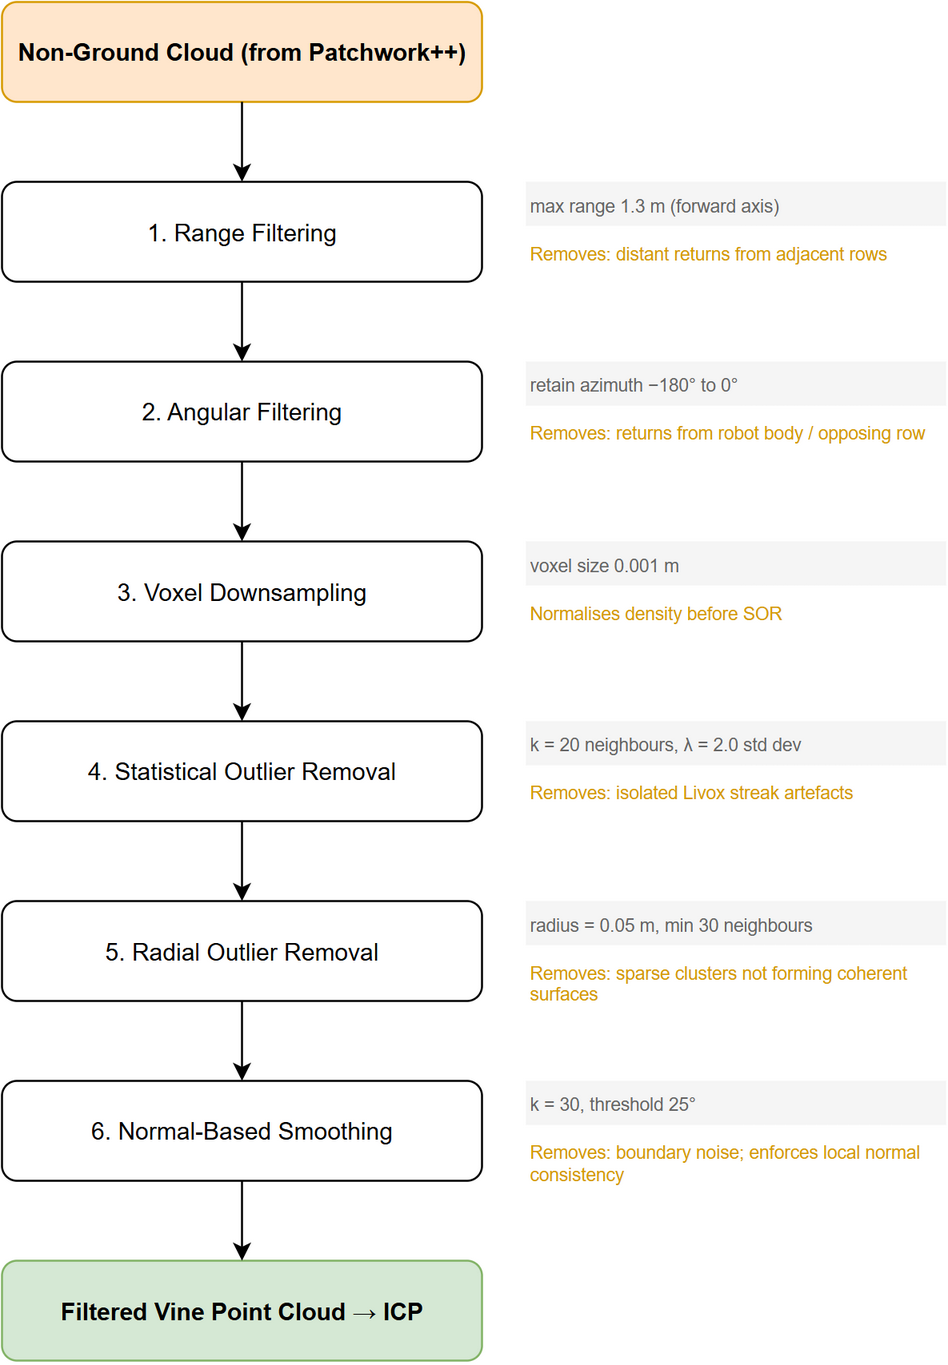
\includegraphics[width=0.75\linewidth]{4-precise-alignment/4-methodology/figures/pa-lidar-filtering}
  \caption{LiDAR point cloud filtering pipeline. Six sequential stages process the
           non-ground Livox cloud to isolate vine wood structure prior to ICP
           registration.}
  \label{fig:pa-lidar-filtering}
\end{figure}

The six sequential stages are described below.

\textbf{Range filtering.} Points beyond a maximum range of 1.3\,m from the sensor are discarded. This restricts the cloud to the area of the target vine, removing distant returns from adjacent rows and structures that do not exist in the 3DGS reference model.

\textbf{Angular filtering.} Points in the azimuthal range from $-180^{\circ}$ to $0^{\circ}$ are retained; returns outside this half-space are discarded.
This step exploits the known mounting orientation of the Livox sensor to exclude returns from the robot body and from the vineyard row that the robot is not currently targeting.

\textbf{Voxel downsampling.} The angular-filtered point cloud is downsampled using a voxel grid filter with voxel side length 0.001\,m. This normalises point density before subsequent filtering stages, ensuring that the statistical outlier removal threshold operates on a spatially uniform cloud rather than being biased by density variations inherent to the non-repetitive scan pattern.

\textbf{Statistical outlier removal.} Each point is evaluated against its $k$-nearest neighbourhood; points whose mean neighbour distance exceeds the population mean by more than $\lambda$ standard deviations are classified as outliers and removed. With $k = 20$ and $\lambda = 2.0$, Operating on the voxel-downsampled cloud ensures that the mean-plus-$2\sigma$ threshold targets outliers rather than points in naturally sparse scan regions.

\textbf{Radial outlier removal.} A spherical neighbourhood of radius 0.05\,m around each point is examined; points with fewer than 30 neighbours within that radius are discarded.
This pass targets point clusters that are spatially consistent at the individual-point level but are too isolated to form part of a coherent surface.

\textbf{Normal-based smoothing.} Surface normals are estimated for each point from its 30 nearest neighbours. Points whose estimated normal deviates by more than $25^{\circ}$ from the local consensus are discarded, enforcing normal consistency across the retained surface. This smoothing pass reduces boundary effects and the influence of surface noise on the ICP correspondence stage.

The parameters for the LiDAR preprocessing pipeline are summarised in \cref{tab:pa-lidar-params}.

\begin{table}[htbp]
  \centering
  \caption{LiDAR pipeline parameters.}
  \label{tab:pa-lidar-params}
  \begin{tabularx}{\textwidth}{l l X}
    \toprule
    \textbf{Parameter} & \textbf{Value} & \textbf{Description} \\
    \midrule
    \multicolumn{3}{l}{\textit{Patchwork++ ground segmentation}} \\
    \midrule
    Sensor height          & 0.88\,m        & Mounting height of the Livox sensor above the ground \\
    Distance threshold     & 0.125\,m       & Maximum deviation from the fit plane to be classified as ground \\
    Seed threshold         & 0.5\,m         & Height threshold for initial ground seed selection \\
    Fitting iterations     & 3              & Number of plane-fitting iterations per annular patch \\
    Processing range       & 0.1--3.0\,m    & Minimum and maximum range included in ground estimation \\
    RNR                    & Enabled        & Ring-wise Normal-based Removal \\
    RVPF                   & Enabled        & Ring-wise Vertical Point Filtering \\
    \midrule
    \multicolumn{3}{l}{\textit{Point cloud filtering}} \\
    \midrule
    Range filter max range              & 1.3\,m                    & Maximum range from sensor along the forward axis \\
    Angular filter range                & $-180^{\circ}$ to $0^{\circ}$ & Retained azimuthal range \\
    Voxel downsample size               & 0.001\,m                  & Voxel side length for density normalisation prior to SOR \\
    Statistical outlier $k$             & 20                        & Neighbourhood size for statistical outlier removal \\
    Statistical outlier $\lambda$       & 2.0                       & Standard deviation multiplier for the outlier threshold \\
    Radial outlier radius               & 0.05\,m                   & Neighbourhood radius for radial outlier removal \\
    Radial outlier min neighbours       & 30                        & Minimum neighbours within the search radius \\
    Normal smooth $k$                   & 30                        & Neighbourhood size for normal estimation \\
    Normal smooth threshold             & $25^{\circ}$              & Maximum normal deviation for smoothing-stage retention \\
    \bottomrule
  \end{tabularx}
  % TODO: verify all parameter values and add justifications
\end{table}

% ---------------------------------------------------------------
\subsection{ICP Registration Against the 3DGS Model}
\label{subsec:pa-icp-registration}
% ---------------------------------------------------------------

Both the stereo and LiDAR preprocessing branches deliver a filtered source point cloud to a shared Generalised ICP (GICP) registration module, developed for this work, which aligns the sensor observation against a fixed target point cloud extracted from the 3DGS model. The registration procedure is as follows.

\textbf{(a) Initial pose.} The initial pose estimate, obtained from the SLAM system (\cref{sec:slam-methodology}), is represented as a $4 \times 4$ homogeneous transformation matrix in $SE(3)$, encoding the rotation and translation of the robot base in the global frame.

\textbf{(b) Target cloud construction.} A single target point cloud is constructed once from the Gaussian means of the 3DGS model, as described in \cref{subsec:pa-reference-model}..

\textbf{(c) Neighbourhood perturbation.} To mitigate sensitivity to the accuracy of the initial SLAM pose, the pipeline generates N candidate initial poses by applying small rigid-body perturbations to the initial estimate $T_0$. Each perturbed pose $T_k$ is formed by right-multiplying $T_0$ with a perturbation matrix $\Delta T_k$:
%
\begin{equation}
    T_k = T_0 \cdot \Delta T_k, \qquad k = 0, \ldots, N-1.
    \label{eq:perturbation}
\end{equation}
%
Right-multiplication ensures that perturbations are applied in the body frame of the robot, so that translations and rotations act along the robot's local axes rather than the global frame axes. The N hypotheses are organised into five groups according to the structure of $\Delta T_k$, as summarised in \cref{tab:pa-perturbation-groups}. The perturbation magnitudes $\delta_t$ (translation) and $\delta_r$ (rotation) are configurable parameters whose values are reported in \cref{tab:pa-icp-params}. The perturbation scheme and subsequent hypothesis selection are illustrated in \cref{fig:pa-icp-candidates}.

\begin{table}[htbp]
  \centering
  \caption{Perturbation hypothesis groups. Each group defines a class of rigid-body perturbation applied to the initial pose to generate candidate starting points for GICP registration.}
  \label{tab:pa-perturbation-groups}
  \begin{tabularx}{\textwidth}{l l X}
    \toprule
    \textbf{Group} & \textbf{Count} & \textbf{Description} \\
    \midrule
    Orig & 1  & Nominal (unperturbed) pose; $\Delta T_0 = I_{4\times4}$ \\
    A    & 6  & Axis-aligned translations along $\pm x$, $\pm y$, $\pm z$ at half the nominal magnitude ($\delta_t / 2$) \\
    B    & 4  & Cardinal-direction translations in the horizontal plane ($+x$, $-x$, $+y$, $-y$) at the full nominal magnitude ($\delta_t$) \\
    C    & 12 & Compound perturbations combining a diagonal horizontal translation ($\delta_t$) with a yaw rotation ($\pm \delta_r$), sampling the four diagonal directions (NE, SE, SW, NW) with both positive and negative yaw \\
    E    & 12 & Rotation-only perturbations sweeping roll, pitch, and yaw about each axis at both half-magnitude ($\delta_r / 2$) and full magnitude ($\delta_r$), with positive and negative signs \\
    \midrule
    \textbf{Total} & \textbf{35} & \\
    \bottomrule
  \end{tabularx}
\end{table}

\begin{figure}[htbp]
  \centering
  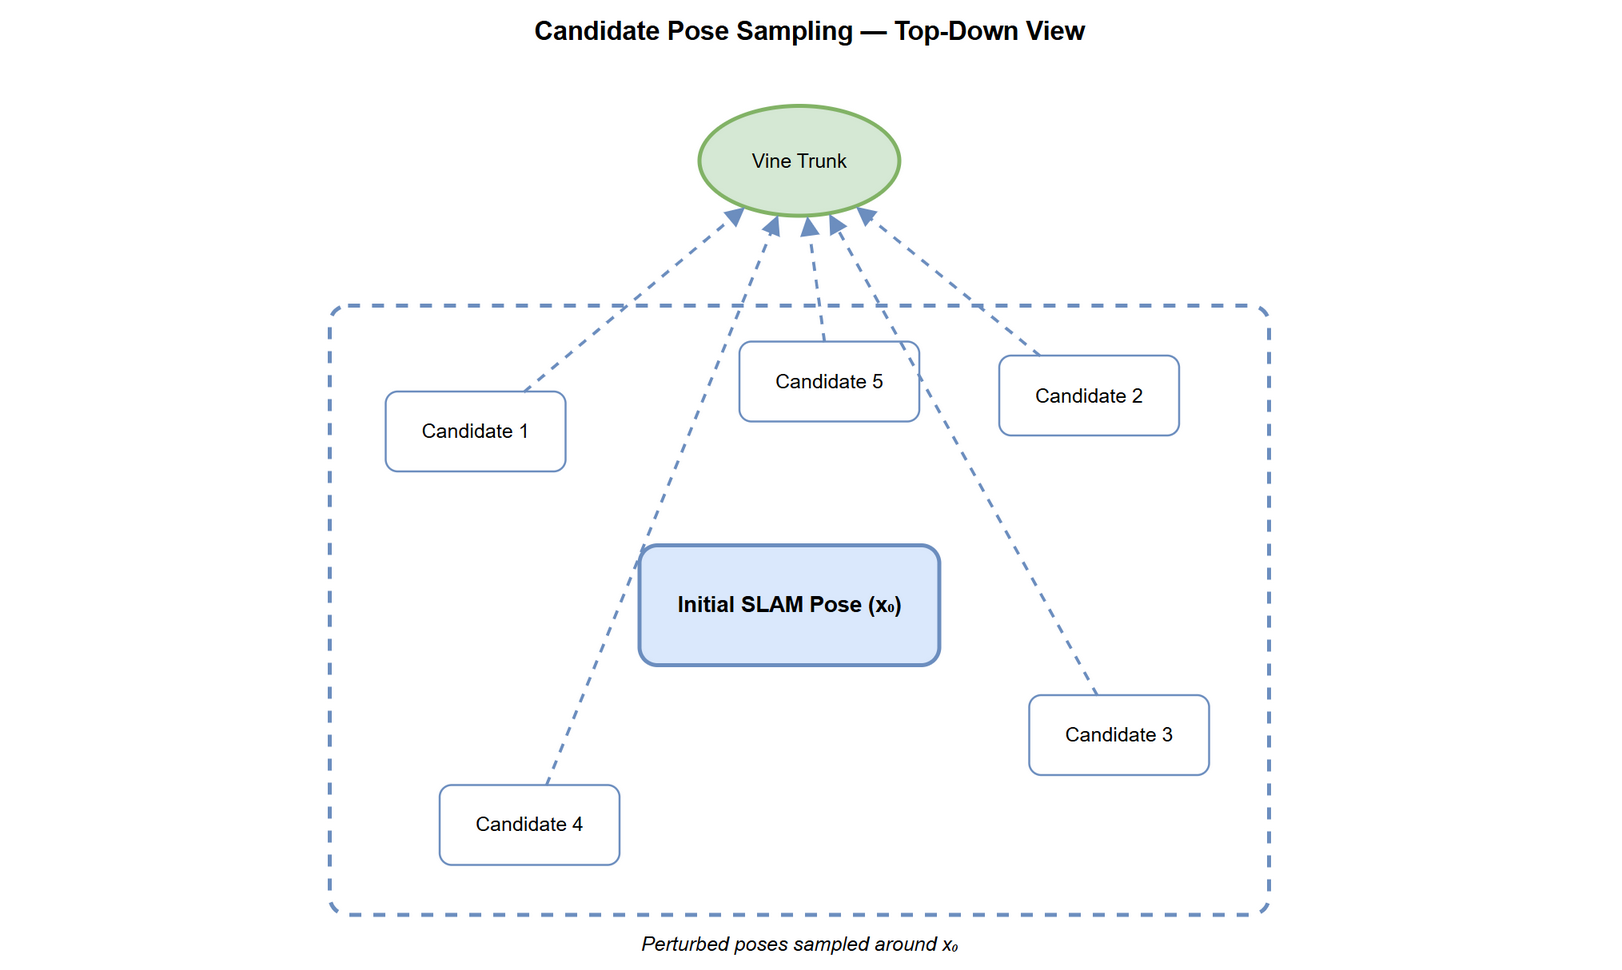
\includegraphics[width=\linewidth]{4-precise-alignment/4-methodology/figures/pa-icp-candidates}
  \caption{Candidate pose sampling scheme (top-down view). Thirty-five candidate poses are generated
           by applying structured rigid-body perturbations (Orig and Groups~A, B, C,~and~E; \cref{tab:pa-perturbation-groups})
           to the initial SLAM pose; each hypothesis is registered independently against the
           target point cloud extracted from the 3DGS model. The hypothesis achieving the highest
           fitness score above the acceptance threshold (lowest RMSE as a tiebreaker) is selected
           as the final alignment.}
  \label{fig:pa-icp-candidates}
\end{figure}

\textbf{(d) Downsampling.} Both the source cloud and the target cloud are downsampled using a voxel grid filter with voxel side length $v = 0.0075$\,m. The target cloud may have been pre-downsampled during construction (see \cref{subsec:pa-reference-model}); the additional voxel filter ensures a consistent resolution across registration runs. This step reduces the computational cost of each GICP iteration while retaining sufficient geometric detail for convergence.

\textbf{(e) GICP.} GICP~\cite{segalGeneralizedICP2009} is run between the downsampled source cloud and the downsampled target cloud using the \texttt{registration\_generalized\_icp} function from Open3D~\cite{zhouOpen3DModernLibrary2018}. Unlike standard point-to-point ICP, GICP models local surface structure by estimating covariance matrices in the neighbourhood of each point in both the source and target clouds, using a hybrid KD-tree neighbourhood search. The generalised objective incorporates these covariances to perform an effective plane-to-plane alignment, making it more robust to incorrect correspondences than the point-to-point formulation~\cite{segalGeneralizedICP2009}. Each of the 35 perturbed initial poses is used as the starting transformation for an independent GICP run. Each run applies a two-phase graduated loss strategy with an accumulated rotation constraint, as described below; the governing parameters are summarised in \cref{tab:pa-icp-params}.

\textbf{(f) Hypothesis selection.} After all 35 GICP runs complete, hypotheses with a fitness score below a threshold of 0.8 are rejected, where fitness is defined as the ratio of accepted correspondences to total source points. A fitness score of 0.8 requires that at least 80\% of the source points find a geometrically consistent correspondence in the target cloud, ensuring that the accepted alignment is supported by the majority of the observed structure rather than a minority subset. Among the remaining hypotheses, the result with the highest fitness score is selected as the final alignment, with the lowest RMSE used as a tiebreaker when fitness scores are equal.

The output of the registration stage is a result object containing the estimated transformation matrix, the fitness score, the point-to-point RMSE, and the accepted correspondence set.

\subsubsection*{Graduated Loss Strategy and Rotation Constraint}
\label{subsubsec:pa-graduated-icp}

Applying a single robust loss function throughout an ICP run creates a tension between two competing requirements. In early iterations, the source and target clouds are poorly aligned, so most point correspondences carry large residuals regardless of their geometric validity; aggressive outlier rejection at this stage can discard informative correspondences from thin structures such as branches and support wires, impeding convergence. Once broad alignment is achieved, the residuals that remain large arise from genuinely poor correspondences (edge noise, structural ambiguity), and strong suppression is desirable to lock the solution onto reliable inlier correspondences. A graduated loss strategy addresses this tension by using a permissive loss in the first phase and switching to an aggressive loss in the second. The complete constrained registration loop is illustrated in \cref{fig:pa-graduated-icp}.

\begin{figure}[htbp]
  \centering
  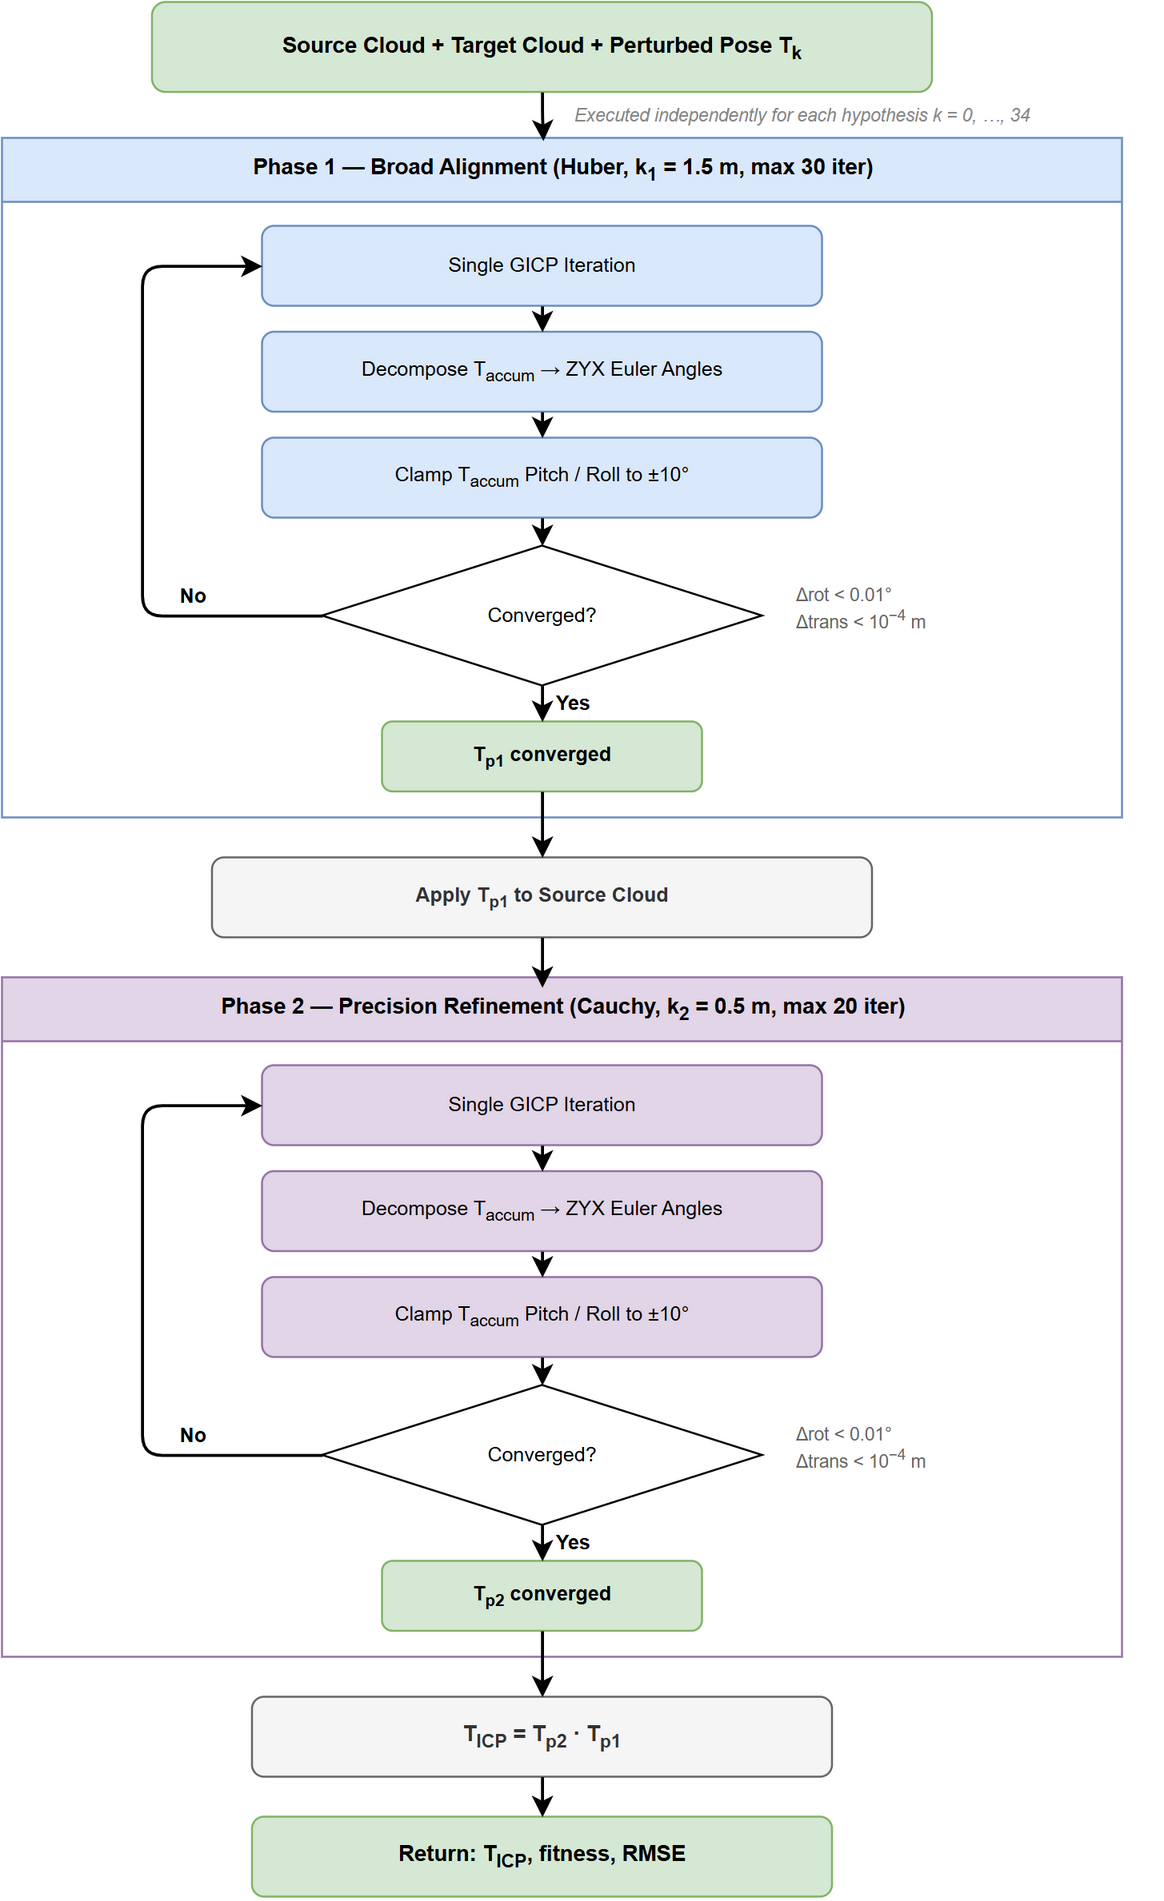
\includegraphics[width=0.75\linewidth]{4-precise-alignment/4-methodology/figures/pa-graduated-icp}
  \caption{Graduated GICP registration loop for a single perturbation hypothesis.
           Phase~1 uses a Huber loss ($k_1 = 1.5$\,m) for broad alignment;
           Phase~2 switches to a Cauchy loss ($k_2 = 0.5$\,m) for precision
           refinement. Both phases apply a rotation constraint
           that clamps the total accumulated pitch and roll correction to $\pm 10^{\circ}$.
           The final transformation is composed as
           $T_{\text{ICP}} = T_{\text{p2}} \cdot T_{\text{p1}}$.}
  \label{fig:pa-graduated-icp}
\end{figure}

\paragraph{Phase 1: Huber loss (broad alignment).}
The first phase uses a Huber robust loss function:
%
\begin{equation}
    \rho_H(r) =
    \begin{cases}
        \tfrac{1}{2} r^2                       & \text{if } |r| \leq k_1, \\
        k_1 \!\left(|r| - \tfrac{1}{2} k_1\right) & \text{otherwise,}
    \end{cases}
    \label{eq:huber-loss}
\end{equation}
%
where $r$ is the residual distance for a correspondence and $k_1 = 1.5$\,m is the scale parameter. Below $k_1$ the Huber loss is purely quadratic; above $k_1$ it grows linearly rather than being truncated entirely. The large value of $k_1$ means that the transition to linear growth occurs late, so the majority of correspondences, even those with substantial residuals early in registration, contribute a non-zero gradient and keep the optimisation from stalling. Phase~1 runs for a maximum of 30 iterations per hypothesis.

\paragraph{Phase 2: Cauchy loss (precision refinement).}
After Phase~1 brings the clouds into approximate alignment, the second phase switches to a Cauchy robust loss:
%
\begin{equation}
    \rho_C(r) = \frac{k_2^2}{2} \ln\!\left(1 + \left(\frac{r}{k_2}\right)^2\right),
    \label{eq:cauchy-loss}
\end{equation}
%
where $k_2 = 0.5$\,m. The Cauchy loss grows logarithmically for large residuals, so correspondences whose residuals exceed $k_2$ by even a modest factor are strongly down-weighted. With $k_2 = 0.5$, a residual of $0.75$\,m (i.e.\ $1.5\,k_2$) is already in the aggressive suppression regime, making Phase~2 sensitive only to the tightest inlier set. The Phase~1 converged transformation $T_{\text{p1}}$ is applied to the source cloud in place before Phase~2 begins, so that Phase~2 refines from the Phase~1 result. Phase~2 runs for a maximum of 20 iterations per hypothesis. The final combined transformation is:
%
\begin{equation}
    T_{\text{ICP}} = T_{\text{p2}} \cdot T_{\text{p1}},
    \label{eq:icp-combined}
\end{equation}
%
where $T_{\text{p2}}$ is the refinement returned by Phase~2.

\paragraph{Rotation constraint.}
Open3D's \texttt{registration\_generalized\_icp} provides no built-in mechanism for constraining the per-iteration correction. A custom iterative loop therefore replaces the library's internal iteration for both phases: at each step, a single GICP iteration is executed and the accumulated correction transform $T_{\text{accum}}$ (the total ICP-introduced change relative to the current phase's starting pose) is decomposed into ZYX Euler angles. The pitch and roll components of $T_{\text{accum}}$ are clamped to $\pm 10^{\circ}$; yaw and all three translation components remain unconstrained. Because the clamping is applied to $T_{\text{accum}}$ rather than to the absolute pose, it constrains only the correction introduced by ICP and preserves any pitch or roll present in the initial estimate. This is appropriate because the robot operates on approximately level terrain, so large pitch or roll corrections are more likely to be registration artefacts than genuine pose refinements.

Convergence in the constrained loop is declared when the incremental rotation between successive steps falls below $0.01^{\circ}$ and the incremental translation falls below $10^{-4}$\,m, or when the maximum iteration count for that phase is reached. Phase~1 clamps $T_{\text{accum}}$ relative to the initial perturbed pose; Phase~2 clamps $T_{\text{accum}}$ relative to the Phase~1 converged pose.

The parameters for the GICP registration stage are summarised in \cref{tab:pa-icp-params}.

\begin{table}[htbp]
  \centering
  \caption{GICP registration parameters.}
  \label{tab:pa-icp-params}
  \begin{tabularx}{\textwidth}{@{} >{\raggedright}p{0.27\textwidth} >{\raggedright}p{0.20\textwidth} >{\raggedright\arraybackslash}X @{}}
    \toprule
    \textbf{Parameter} & \textbf{Value} & \textbf{Description} \\
    \midrule
    Perturbation hypotheses         & 35                  & Total candidate poses: 1 nominal (Orig) + 34 perturbations (Groups~A, B, C, and~E; \cref{tab:pa-perturbation-groups}) \\
    Translation perturbation ($\delta_t$) & $0.10$\,m & Full magnitude used by Groups~B and~C; Group~A uses $\delta_t / 2 = 0.05$\,m \\
    Rotation perturbation ($\delta_r$)    & $10^{\circ}$ & Full magnitude used by Group~C (yaw component); Group~E uses both $\delta_r / 2 = 5^{\circ}$ and $\delta_r$ \\
    Voxel grid size ($v$)           & 0.0075\,m           & Downsampling resolution applied to source and target clouds \\
    GICP backend                    & Open3D              & \texttt{registration\_generalized\_icp}; generalised ICP implementation from Open3D~\cite{zhouOpen3DModernLibrary2018} \\
    Phase~1 loss (LiDAR)            & Huber, $k_1 = 1.5$\,m & Broad alignment phase; soft outlier rejection (\cref{eq:huber-loss}) \\
    Phase~1 max iterations          & 30                  & Per hypothesis \\
    Phase~2 loss (LiDAR)            & Cauchy, $k_2 = 0.5$\,m & Precision refinement phase; aggressive outlier rejection (\cref{eq:cauchy-loss}) \\
    Phase~2 max iterations          & 20                  & Per hypothesis \\
    Max correspondence distance     & 0.15\,m             & Maximum point-pair distance for correspondence acceptance \\
    Rotation constraint (LiDAR)     & $\pm 10^{\circ}$ pitch/roll & Clamp on total accumulated ICP correction; yaw unconstrained \\
    Constrained convergence: rotation    & $0.01^{\circ}$ & Inter-step rotation change threshold \\
    Constrained convergence: translation & $10^{-4}$\,m   & Inter-step translation change threshold \\
    Fitness threshold               & 0.8                 & Minimum fitness score for hypothesis acceptance \\
    \bottomrule
  \end{tabularx}
\end{table}

% ---------------------------------------------------------------
\subsection{Coordinate Frames and Pose Correction}
\label{subsec:pa-pose-correction}
% ---------------------------------------------------------------

The ICP registration stage returns a rigid transformation expressed in the sensor frame (that is, the frame of the camera or LiDAR sensor from which the source cloud was acquired). Before this result can be applied to the robot's localisation, it must be expressed in the base-link frame that serves as the canonical reference for all downstream planning and control components. It must also be introduced into the ROS~2 transform tree~\cite{macenskiRobotOperatingSystem2022} without disturbing the SLAM system's own transform publications.

\subsubsection*{Coordinate Frame Hierarchy}

The coordinate frame hierarchy used throughout this system is:
\[
  \texttt{local\_enu} \to \texttt{map} \to \texttt{odom} \to \texttt{base\_link} \to \texttt{sensor\_frame},
\]
where \texttt{local\_enu} is the ENU-anchored global frame, \texttt{map} and \texttt{odom} are the frames published by the SLAM system, \texttt{base\_link} is the robot body frame, and \texttt{sensor\_frame} is the frame of whichever sensor produced the source cloud. The static transforms between \texttt{base\_link} and the sensor frames are fixed by the mechanical configuration of the platform and are loaded at launch from the robot description.

\subsubsection*{TF Correction Mechanism}

A custom TF correction mechanism developed for this work inserts a correction frame into the transform tree without modifying any of the transforms published by the SLAM system. The ICP result provides the correction in the sensor frame, $T_{\mathrm{correction, sensor}}$. To express this correction at the level of the base link, the following composition is applied:
%
\begin{equation}
    T_{\mathrm{correction, base}} =
        T_{\mathrm{base} \to \mathrm{sensor}}^{-1}
        \cdot T_{\mathrm{correction, sensor}}
        \cdot T_{\mathrm{base} \to \mathrm{sensor}},
    \label{eq:tf-correction}
\end{equation}
%
where $T_{\mathrm{base} \to \mathrm{sensor}}$ is the fixed extrinsic transform from the base link to the sensor frame. The resulting base-frame correction is then inserted into the appropriate location in the transform chain and published as a static transform, as illustrated in \cref{fig:pa-tf-correction}.

\begin{figure}[htbp]
  \centering
  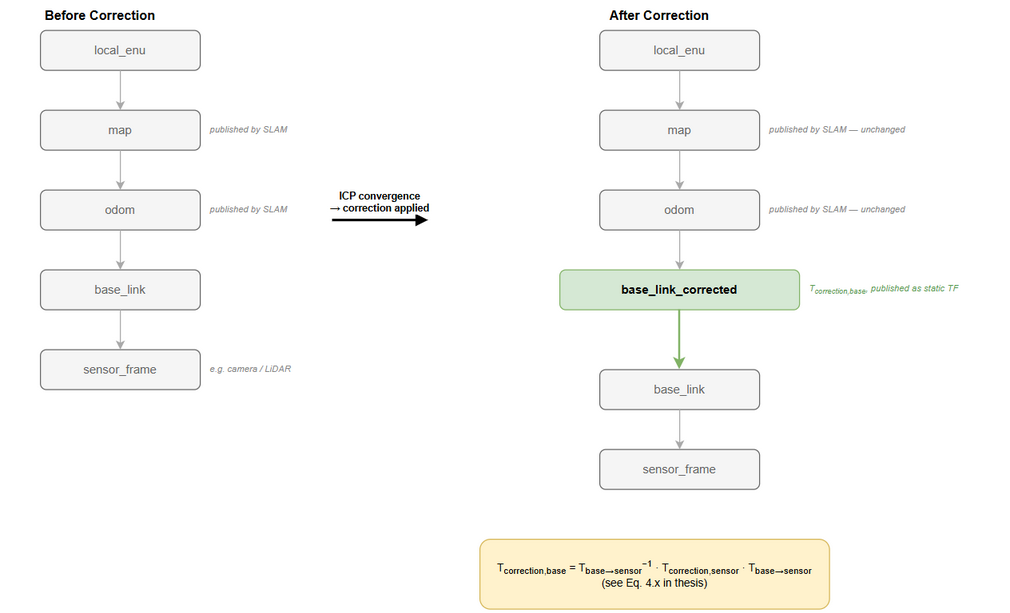
\includegraphics[width=\linewidth]{4-precise-alignment/4-methodology/figures/pa-tf-correction}
  \caption{ROS~2 TF transform tree before (left) and after (right) insertion of the pose
           correction frame. The correction is introduced between the SLAM-published
           \texttt{odom} frame and downstream planning frames without modifying the SLAM
           system's own publications. $T_{\mathrm{correction,base}}$ is derived from the
           ICP result via the extrinsic $T_{\mathrm{base} \to \mathrm{sensor}}$
           (\cref{eq:tf-correction}).}
  \label{fig:pa-tf-correction}
\end{figure}

Because the correction is published as a static transform, it does not require a continuous update loop and is non-disruptive to the SLAM publishers. The correction mechanism supports both automatic triggering (applied immediately upon successful ICP convergence) and manual triggering, in which the operator confirms before the correction is broadcast to the transform tree. The appropriate mode is selected at launch via a configuration parameter.

% ---------------------------------------------------------------
\subsection{Pipeline Execution Model}
\label{subsec:pa-execution-model}
% ---------------------------------------------------------------

Each precise alignment request is encapsulated as an ordered sequence of command objects following the Command design pattern. Each processing stage (depth estimation, point cloud preprocessing, target cloud extraction, ICP registration, and pose correction) is implemented as an \texttt{AsyncCommand} with a well-defined input contract and output contract. Commands are submitted to an asynchronous task queue, which executes them sequentially within a dedicated worker thread pool. This design decouples the processing pipeline from the ROS~2 executor event loop: computationally intensive operations such as FoundationStereo inference and Open3D ICP run in non-blocking threads, avoiding latency spikes in the ROS~2 message-handling callbacks. The execution architecture is illustrated in \cref{fig:pa-execution-model}.

\begin{figure}[htbp]
  \centering
  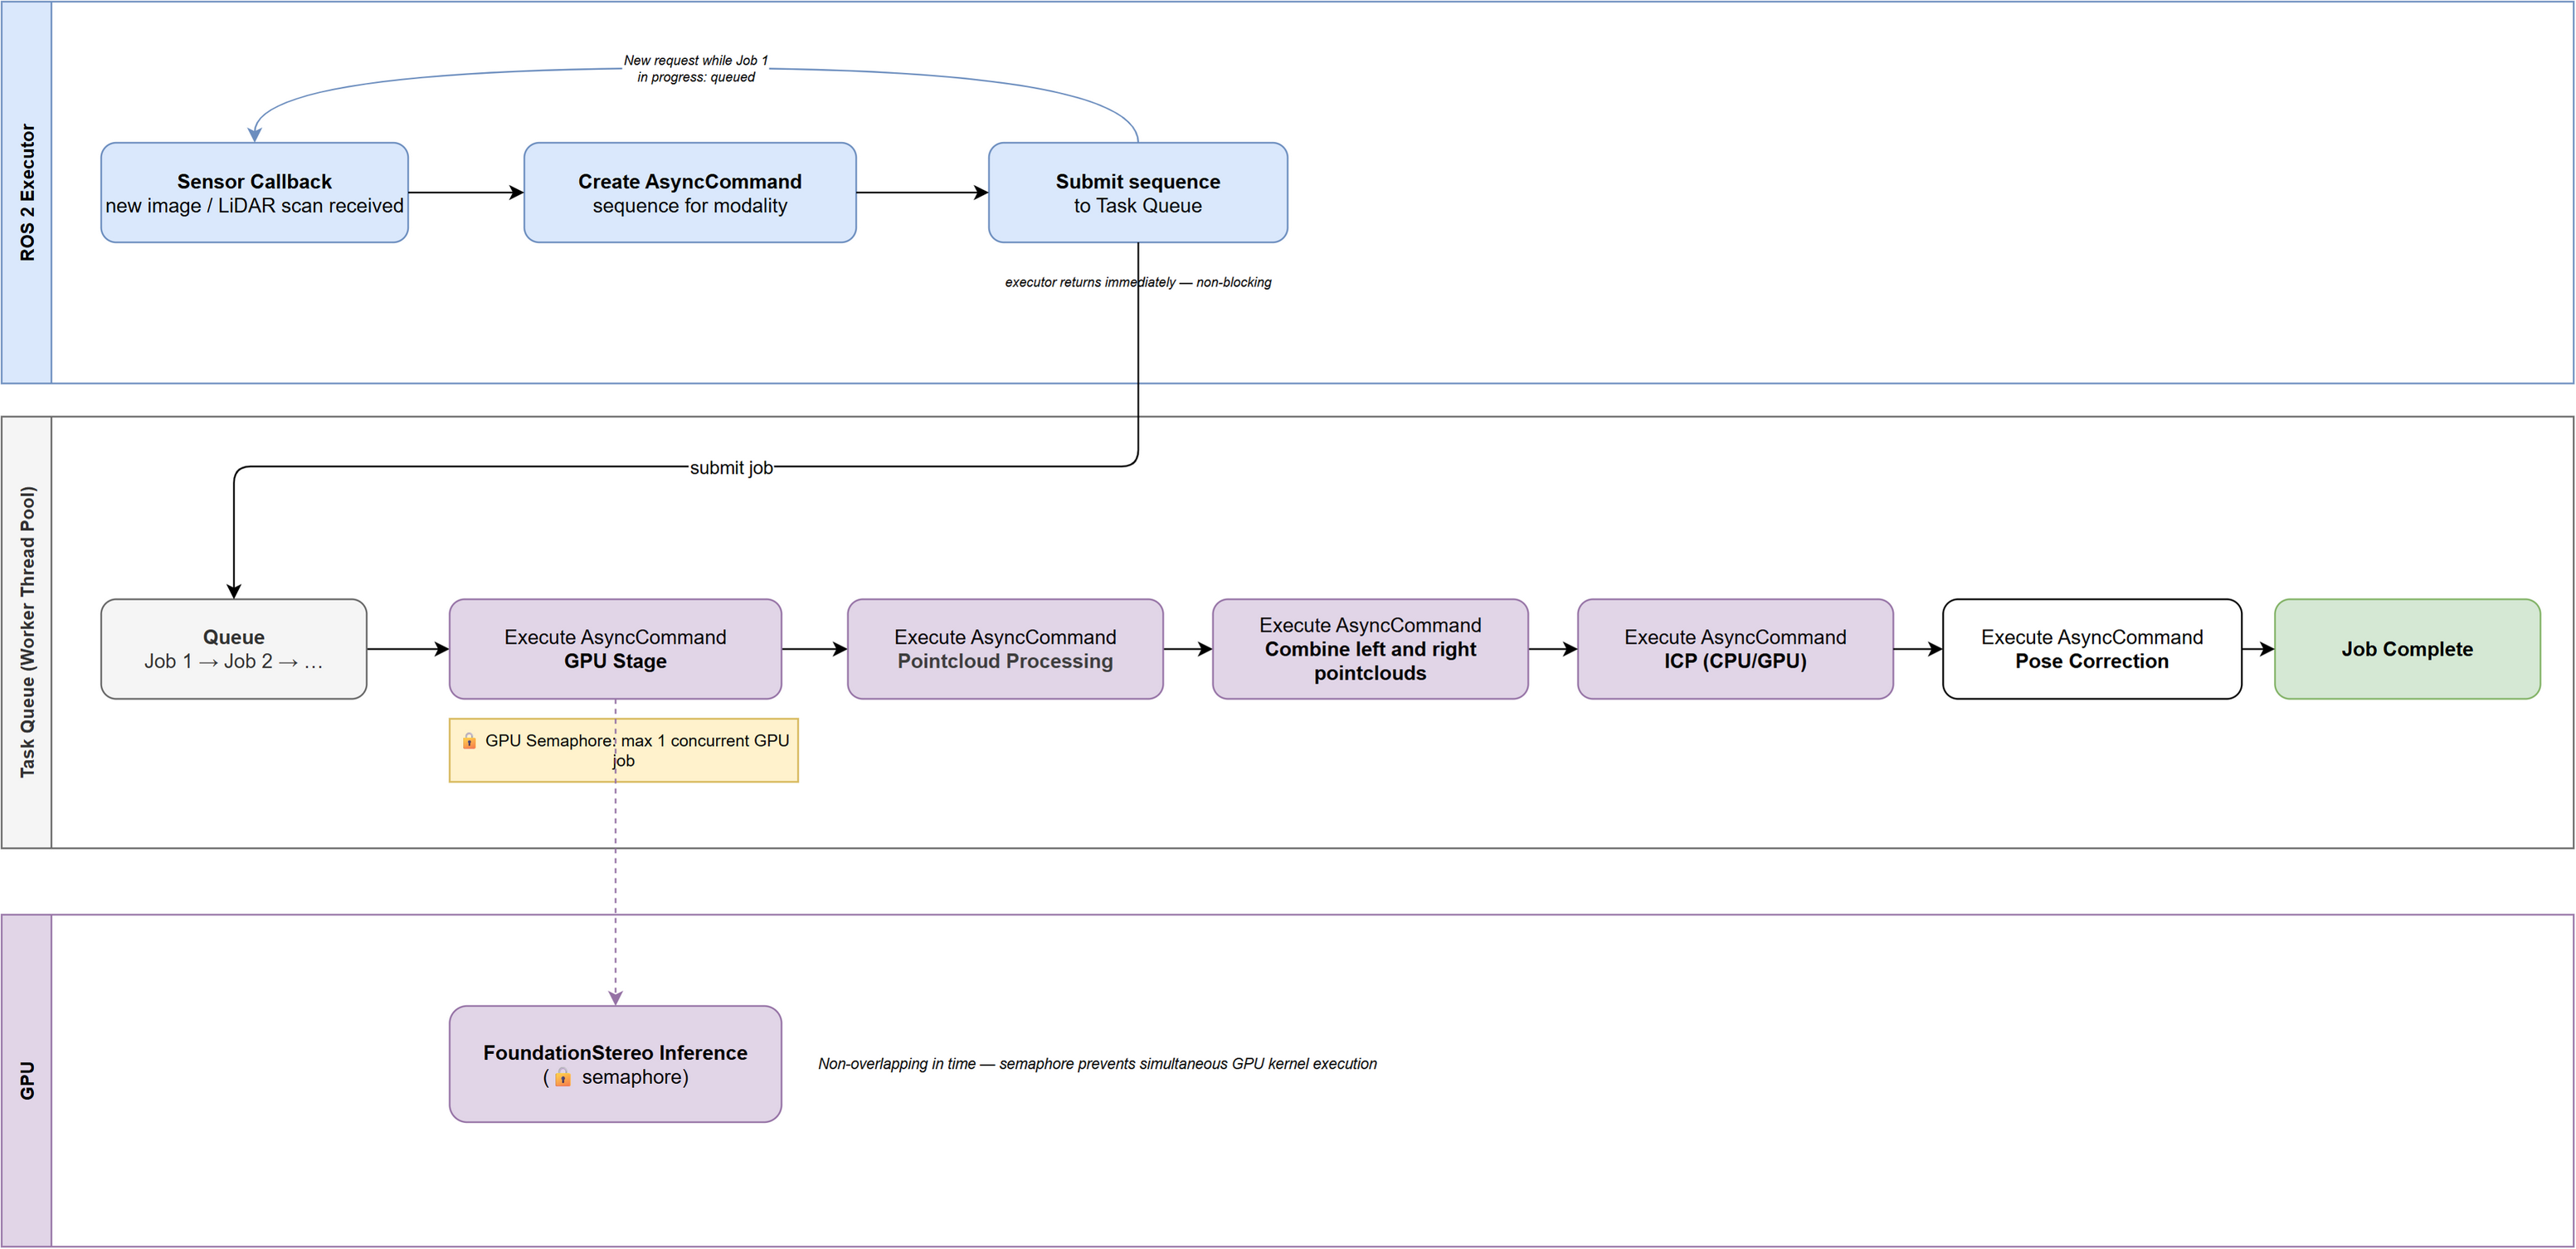
\includegraphics[width=\linewidth]{4-precise-alignment/4-methodology/figures/pa-execution-model}
  \caption{Pipeline execution model for the stereo modality. The LiDAR pipeline
           follows the same structure with modality-specific command steps.}
  \label{fig:pa-execution-model}
\end{figure}

The GPU-resident FoundationStereo inference stage is governed by a semaphore-based concurrency guard that prevents simultaneous kernel execution from exceeding available GPU memory. Target cloud extraction from the 3DGS model reads Gaussian mean positions on the CPU and is not subject to this guard. When a new alignment request arrives while a prior job is still processing, it enters the pipeline as soon as the first stage becomes available; the stages are pipelined such that a subsequent job may begin executing a stage once the preceding job has advanced beyond it, allowing multiple jobs to be processed concurrently at different stages. This execution model supports both the stereo and LiDAR pipelines without modification, as the modality-specific processing difference is captured entirely within the command sequence submitted for each observation type.

The preceding subsections have described the complete precise alignment pipeline: sensor preprocessing for both stereo and LiDAR observations, target point cloud extraction from the 3DGS model, GICP registration with neighbourhood perturbation, and pose correction. The following subsection describes the experimental setup designed to evaluate the LiDAR pipeline under controlled conditions. The results of these experiments are presented in \cref{sec:precise-alignment-results}.

% ===============================================================
\subsection{Experimental Setup}
\label{subsec:pa-experimental-setup}
% ===============================================================
% TODO: document the computational resources used for evaluation: (1) robot onboard compute (CPU, GPU, RAM) and (2) local machine specs (CPU, GPU, RAM) used to run evals offline.

This section describes the experimental setup used to evaluate the precise-alignment pipeline. LiDAR and stereo data were recorded simultaneously during each trial; both sensing modalities are therefore evaluated against the same set of trial conditions. Six aspects of the evaluation are described: the test environment, the vine specimen and reference model, the trial design, the construction of initial poses, the evaluation protocol, and the metrics used to validate alignment quality.

% ---------------------------------------------------------------
\subsubsection{Test Environment}
\label{subsubsec:pa-test-environment}
% ---------------------------------------------------------------

Trials were conducted in an indoor laboratory environment. This study is scoped to dormant-season vineyard conditions, in which vines present a leafless, woody skeletal structure. At the time of evaluation, vines in the field retained their autumn foliage, rendering outdoor vineyard environments unsuitable for testing the pipeline under its intended operating conditions. Two dead vine specimens were therefore sourced from a vineyard and mounted side by side on an aluminium support rig fitted with tensioned guide wires, replicating the structural arrangement of a vineyard bay. Although no longer living, the specimens retain their woody trunk and cane structure, which is characteristic of dormant vines and is considered representative of the target scenario.

Outdoor validation was also precluded for a practical reason. The 3DGS reference model was reconstructed from outdoor SfM photogrammetry of the specimen at its original collection site. Subsequent construction at that site has rendered it inaccessible, precluding live-registration trials under the original georeferenced coordinate frame. The specimens were accordingly relocated to the indoor laboratory, where they were mounted on the support rig and the 3DGS model's coordinate system was manually aligned to the laboratory frame. The indoor laboratory therefore served as a controlled proxy environment; outdoor validation under field conditions remains future work.

Several limitations of the indoor evaluation should be noted. First, the dead specimens may exhibit different surface reflectance characteristics compared with living dormant vines; LiDAR return intensity and noise profiles may therefore not be fully representative of field conditions, though the woody geometric structure is preserved. Second, the aluminium support rig introduces structural elements like posts and tensioned wires that are not identical to those found in a real vineyard bay; however, since vineyard bays similarly feature vertical timber posts and tensioned guide wires, the overall structural character of the scene is considered broadly representative. Third, any residual error in the manual alignment of the 3DGS model to the laboratory coordinate system is indistinguishable from pipeline registration error in the reported metrics. The physical arrangement of the laboratory, including the vine specimen, robot platform, and sensor positions, is illustrated in \cref{fig:pa-lab-setup}.

\begin{figure}[htbp]
  \centering
  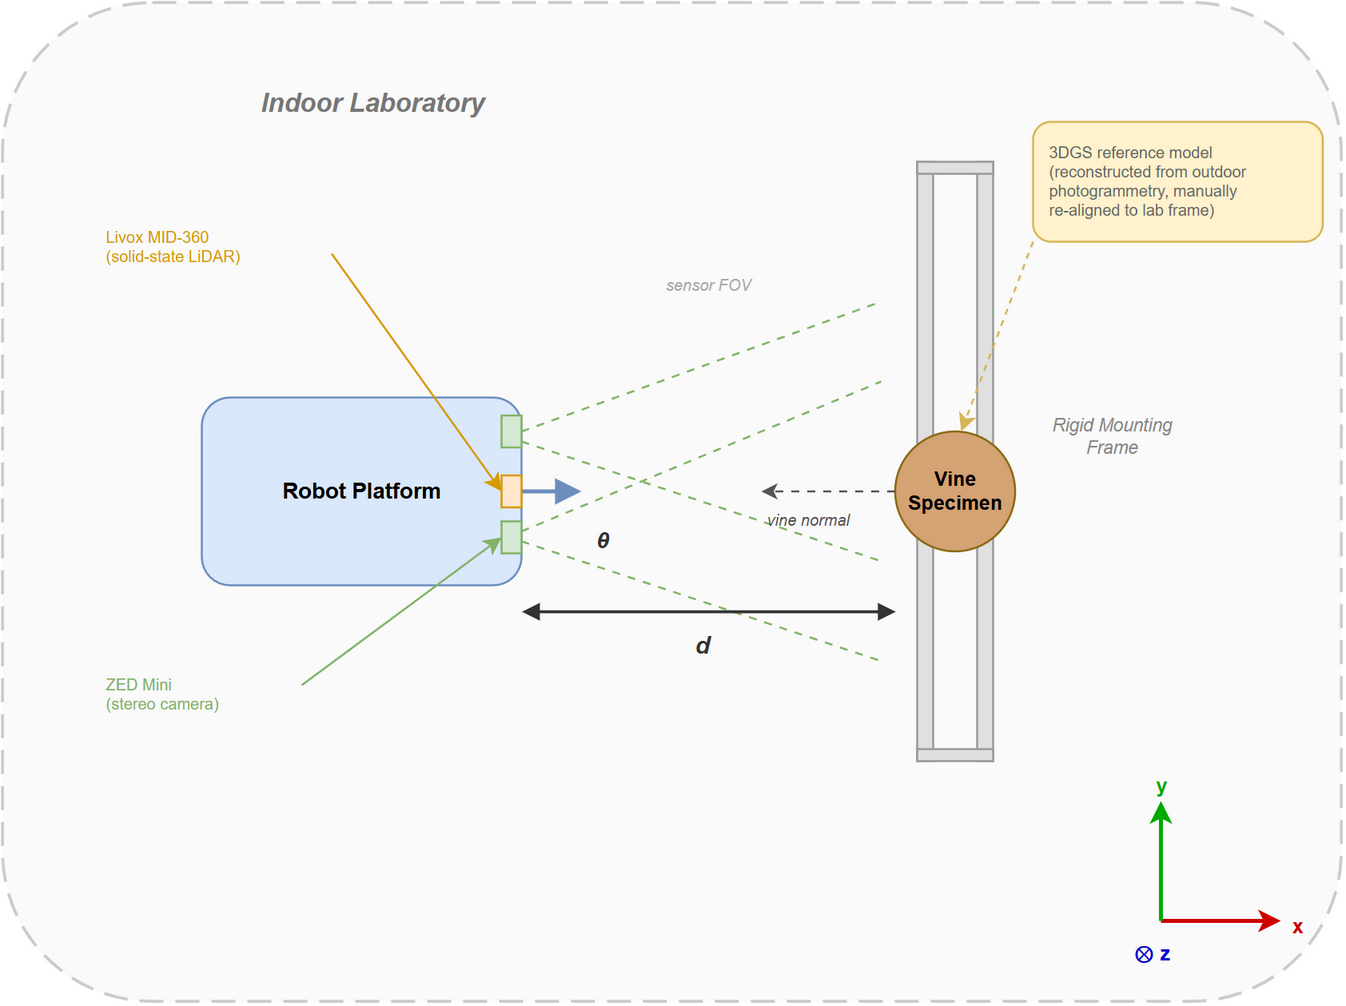
\includegraphics[width=0.85\linewidth]{4-precise-alignment/4-methodology/figures/pa-lab-setup}
  \caption{Physical layout of the indoor laboratory test environment (top-down view).
           The vine specimen is mounted on a rigid frame at a fixed position; the
           robot platform is positioned facing the vine with the Livox LiDAR and
           ZED~Mini stereo camera on its vine-facing side. The distance~$d$ and
           approach angle~$\theta$ define the operating condition for each trial.
           The 3DGS reference model, reconstructed from outdoor photogrammetry,
           was manually re-aligned to the laboratory coordinate frame.}
  \label{fig:pa-lab-setup}
\end{figure}

% ---------------------------------------------------------------
\subsubsection{Vine Specimen and Reference Model}
\label{subsubsec:pa-vine-specimen}
% ---------------------------------------------------------------

A dormant vine specimens were mounted on a rigid physical frame to replicate the vertical trunk structure encountered in a vineyard row. Mounting the specimen on a fixed support ensured that the vine remained stationary throughout all trials, eliminating inter-trial positional drift as a confounding factor.

The 3DGS reference model used for registration was reconstructed from outdoor SfM photogrammetry of the same vine specimen, following the procedure described in \cref{subsec:system-context}. The model is georeferenced in the ENU coordinate frame. For the indoor trials, the model's coordinate system was manually aligned to the laboratory environment to establish a consistent spatial reference between the physical specimen and the model. This alignment provided the common frame of reference required by the registration pipeline.

% ---------------------------------------------------------------
\subsubsection{Trial Design}
\label{subsubsec:pa-trial-design}
% ---------------------------------------------------------------

Trials were organised as a structured evaluation across nine operating conditions defined by two factors: the distance from the sensor to the vine trunk ($d$) and the lateral approach angle ($\theta$) relative to the vine normal. Three levels were selected for each factor: $d \in \{40, 60, 80\}$\,cm and $\theta \in \{-15^{\circ}, 0^{\circ}, {+}15^{\circ}\}$, yielding nine unique conditions that sample the operational envelope at representative points. One additional replicate at the centre condition ($d = 60$\,cm, $\theta = 0^{\circ}$) was included as a repeatability check, resulting in ten trials in total. Because only a single observation is available per non-centre condition, the evaluation is exploratory in nature and does not support formal statistical inference; results characterise pipeline behaviour across the sampled operating conditions rather than quantifying main effects or interactions.

The full trial matrix is summarised in \cref{tab:pa-trial-matrix}; the corresponding spatial layout is shown in \cref{fig:pa-trial-layout}.

\begin{table}[htbp]
  \centering
  \caption{Experimental trial matrix. Each row defines one trial with its distance and angle factor levels. Trial~D60A0r is a replicate of the centre condition (60\,cm, 0$^{\circ}$).}
  \label{tab:pa-trial-matrix}
  \begin{tabularx}{\textwidth}{l c c}
    \toprule
    \textbf{Trial ID} & \textbf{Distance (cm)} & \textbf{Angle ($^{\circ}$)} \\
    \midrule
    D40A-15 & 40 & $-15$ \\
    D40A0   & 40 &    $0$ \\
    D40A15  & 40 & ${+}15$ \\
    D60A-15 & 60 & $-15$ \\
    D60A0   & 60 &    $0$ \\
    D60A15  & 60 & ${+}15$ \\
    D80A-15 & 80 & $-15$ \\
    D80A0   & 80 &    $0$ \\
    D80A15  & 80 & ${+}15$ \\
    D60A0r  & 60 &    $0$ \\
    \bottomrule
  \end{tabularx}
\end{table}

An additional trial at 110\,cm ($d = 110$, $\theta = 0^{\circ}$) was collected during the experimental session but is excluded from analysis. This distance exceeds the stereo pipeline's near-field depth clipping threshold ($z_\text{far} = 1.0$\,m), rendering the condition invalid by design for the stereo modality. To maintain a consistent condition set across both modalities, the D110A0 trial is omitted from all reported results.

\begin{figure}[htbp]
  \centering
  \includegraphics[width=0.7\linewidth]{4-precise-alignment/4-methodology/figures/pa-trial-layout}
  \caption{Spatial layout of the experimental trial conditions (top-down view).
           Nine unique operating conditions are defined by crossing three
           sensor-to-vine distances ($d \in \{40, 60, 80\}$\,cm) with three
           lateral approach angles ($\theta \in \{-15^{\circ}, 0^{\circ},
           {+}15^{\circ}\}$). Trial~D60A0r is a replicate of the centre
           condition. Each blue marker indicates the robot sensor position
           relative to the vine trunk for the corresponding trial.}
  \label{fig:pa-trial-layout}
\end{figure}

% ---------------------------------------------------------------
\subsubsection{Initial Pose Construction}
\label{subsubsec:pa-initial-pose}
% ---------------------------------------------------------------

For each trial, the initial pose was constructed from a manual measurement of the robot's position and orientation relative to the vine specimen. The measurement was encoded as a $4 \times 4$ homogeneous transformation matrix in $SE(3)$ and provided to the localisation pipeline as a substitute for the SLAM-derived initial pose that would be available in a deployed system. This approach allows the registration stage to be evaluated in isolation from the SLAM system, with full control over the initial pose quality.

The distance component was measured with a steel tape measure as the orthogonal distance from a fixed reference point on the vine mounting frame to the LiDAR sensor on the robot. The approach angle was determined by triangulation: from the same reference point, the orthogonal distance to the robot was measured, and a second perpendicular was projected from the robot base back to the vine frame. The distance along the frame between the original reference point and this second intersection point, together with the two perpendicular measurements, defined a triangle from which the approach angle was computed trigonometrically. The measurement geometry is illustrated in \cref{fig:pa-pose-measurement}.

\begin{figure}[htbp]
  \centering
  \includegraphics[width=0.65\linewidth]{4-precise-alignment/4-methodology/figures/pa-pose-measurement}
  \caption{Initial pose measurement geometry (top-down view). The approach
           angle~$\theta$ is determined by triangulation from the vine reference
           point~$P$ on the mounting frame. A perpendicular from the robot sensor
           position~$R$ back to the frame intersects at~$Q$; the lateral offset~$PQ$
           along the frame and the perpendicular distance~$QR$ define a right
           triangle from which $\theta = \arctan(PQ / QR)$ is computed.}
  \label{fig:pa-pose-measurement}
\end{figure}

The manual measurement procedure introduces a positioning uncertainty on the order of $\pm 2$--$3$\,cm in translation and $\pm 2$--$3^{\circ}$ in orientation. The translational uncertainty reflects the combined precision of the tape measure ($\pm 1$\,mm) and the difficulty of consistently identifying the reference point on the frame and the sensor centre on the robot; the angular uncertainty reflects the propagation of these linear measurement errors through the trigonometric angle computation. This uncertainty is substantially smaller than the absolute trajectory error (ATE) observed for the GLIM SLAM system~\cite{koideGLIM3DRangeInertial2024} with GNSS fusion in the outdoor evaluation presented in \cref{sec:slam-results}, where the ATE ranges from 0.07 to 0.17\,m. The manual measurement therefore represents a \emph{more favourable} initial condition than would be encountered in deployment. As a consequence, any alignment failures observed under these laboratory conditions indicate a fundamental limitation of the registration pipeline itself, rather than an artefact of poor initial pose quality.

% ---------------------------------------------------------------
\subsubsection{Evaluation Protocol}
\label{subsubsec:pa-eval-protocol}
% ---------------------------------------------------------------

The per-trial evaluation workflow is illustrated in \cref{fig:pa-eval-flowchart}. For each trial, the pipeline generated 35 perturbation hypotheses distributed around the initial pose, following the perturbation protocol described in \cref{subsec:pa-icp-registration}. Each hypothesis was registered independently using GICP against the target point cloud extracted from the 3DGS model; convergence criteria for the ICP solver are as specified in \cref{tab:pa-icp-params}.

\begin{figure}[htbp]
  \centering
  \includegraphics[width=0.85\linewidth]{4-precise-alignment/4-methodology/figures/pa-eval-flowchart}
  \caption{Per-trial evaluation protocol. The initial pose is perturbed to
           generate 35 candidate hypotheses (Orig and Groups~A, B, C,~and~E), each registered
           independently via GICP. Per-hypothesis fitness and RMSE are recorded;
           hypotheses with fitness below~0.8 are rejected, and the best remaining
           result is selected. Three complementary validation strategies (perturbation convergence consistency, inter-trial consistency, and
           visual overlay) are applied to the serialised results.}
  \label{fig:pa-eval-flowchart}
\end{figure}

The following quantities were recorded for each hypothesis:
%
\begin{itemize}
  \item \textbf{Fitness score}: the ratio of inlier correspondences to the total number of source points;
  \item \textbf{Inlier RMSE}: the root-mean-square error of the accepted inlier correspondences;
  \item \textbf{Estimated transformation}: the $4 \times 4$ matrix in $SE(3)$ representing the registration result;
  \item \textbf{Euler angle decomposition}: a decomposition of the estimated rotation into roll, pitch, and yaw angles, retained for interpretability.
\end{itemize}
%
All per-trial results were serialised to JSON for subsequent analysis. Wall-clock timing was additionally recorded for each trial to assess computational feasibility. The following intervals were measured: total pipeline latency from trigger to corrected pose publication, preprocessing time from raw sensor data to filtered source cloud, and GICP registration time across all 35 hypotheses including hypothesis selection. These timings are reported as mean $\pm$ standard deviation across trials.

% ---------------------------------------------------------------
\subsubsection{Evaluation Metrics and Validation}
\label{subsubsec:pa-eval-metrics}
% ---------------------------------------------------------------

Two primary metrics are used to assess registration quality. The fitness score measures the fraction of source points for which a valid correspondence exists within the maximum correspondence distance threshold; a higher fitness score indicates that a greater proportion of the observed structure is geometrically consistent with the reference model. The inlier RMSE measures the geometric residual of accepted correspondences; lower values indicate tighter point-to-point alignment.

Results are additionally analysed per perturbation group (Orig and Groups~A, B, C, and~E, as defined in \cref{subsec:pa-icp-registration}) to assess whether certain perturbation directions are systematically more or less conducive to convergence. This per-group breakdown reveals whether the pipeline exhibits sensitivity to specific classes of initial pose error.

Three complementary validation strategies are applied. First, \emph{perturbation convergence consistency} assesses whether multiple hypotheses within a single trial converge to similar final poses; large dispersion across hypotheses indicates sensitivity to initialisation rather than a stable registration basin. Second, \emph{inter-trial consistency} examines whether similar factor conditions, for example the same distance at different approach angles, produce comparable fitness and RMSE values, providing evidence that results are not artefacts of a single fortuitous initial pose. Third, \emph{visual overlay} provides qualitative validation by rendering the registered source cloud and target cloud in a common frame for visual inspection of alignment quality. Cross-modal validation, comparing LiDAR and stereo registration outcomes on matched trials, is deferred to the stereo experimental setup section.

Because only a single trial is conducted per non-centre condition, formal statistical tests (e.g.\ ANOVA or interaction-effect estimation) are not applicable. Results are instead presented as a condition-by-condition summary: for each trial, the number of hypotheses exceeding the fitness acceptance threshold, the median and interquartile range (IQR) of fitness and RMSE across accepted hypotheses, and the spread of the recovered transformation components. Cross-condition trends, for example whether fitness degrades with increasing distance or whether oblique angles produce higher RMSE variability, are discussed qualitatively. If the replicate pair (D60A0 and D60A0r) yields consistent results, this is noted as evidence of repeatability; discrepancies are discussed.

\paragraph{Limitations.}
No external six-degree-of-freedom ground truth was available for these trials. The fitness score and inlier RMSE are \emph{internal} registration metrics: they measure how well the source cloud matches the target cloud, but do not directly measure whether the recovered pose corresponds to the robot's true physical pose. A high fitness score is necessary but not sufficient for correct alignment, since ICP can converge to a local minimum that achieves good geometric consistency without recovering the true transformation. Visual overlay provides a qualitative cross-check against gross misalignment, and the consistency of results across the 35 perturbation hypotheses provides evidence that the registration basin is stable. However, the results should be interpreted as evidence of geometric consistency between the sensor observation and the 3DGS reference model, rather than as a direct measurement of absolute pose accuracy. Outdoor validation with surveyed reference poses or a motion capture system would be required to quantify absolute accuracy and remains future work.